\section{Simulation and Observations}
In this section we make use of our model by simulating it for various cases. First we will demonstrate some basic dynamics based on the impact of dissipation $\lambda$, desired velocities $u_i$, and interaction $A$. Next we will focus on collective behavior, and present formations such as lane and stripe formations for counter and cross flows respectively. Some insights are provided on the relationship between the parameters, Hamiltonian, and the collective behavior.

The model parameters defined for the simulation are the same as defined in \autoref{code:model_init}. Any changes made would be mentioned within their respective cases. For reproducibility and comparison, each simulation starts with the same arrangement of pedestrians on the xy-plane as shown in 
\begin{figure}[H]
    \centering
    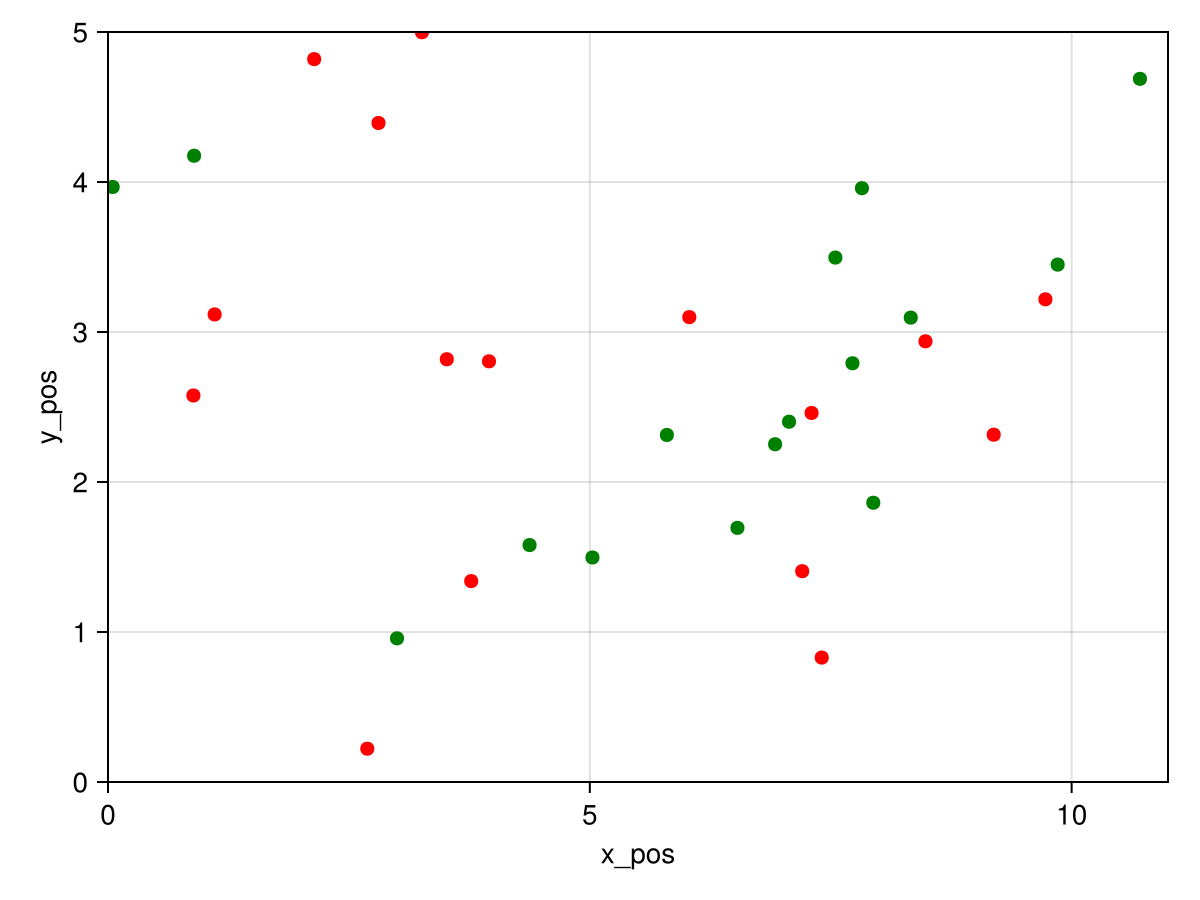
\includegraphics[width=0.55\textwidth]{figures/start_pos.png}
    \caption{Starting positions of pedestrians.}
    \label{plot:starting_pos}
\end{figure}
The color in \autoref{plot:starting_pos} distinguishes between the desired speeds of the pedestrians, which is only relevant for flows that are not unidirectional, as will be shown in \autoref{section:collective}. In the cases of unidirectional flow or where the direction is irrelevant, the color for all is the same.

\subsection{Basic Dynamics}
This section serves to illustrate how the changes in the parameters affect the dynamics of the model, although none of the dynamics presented in the model are realistic, the diagrams provide a way to think about the dynamics of the model based on the changes in the parameter.
\pagebreak
\begin{itemize}
    \item \textbf{No desired velocity ($u_i = \begin{bmatrix} 0 & 0 \end{bmatrix}$) with dissipation ($\lambda > 0$):}
\begin{figure}[H]
    \centering
    \begin{subfigure}{\textwidth}
        \centering
        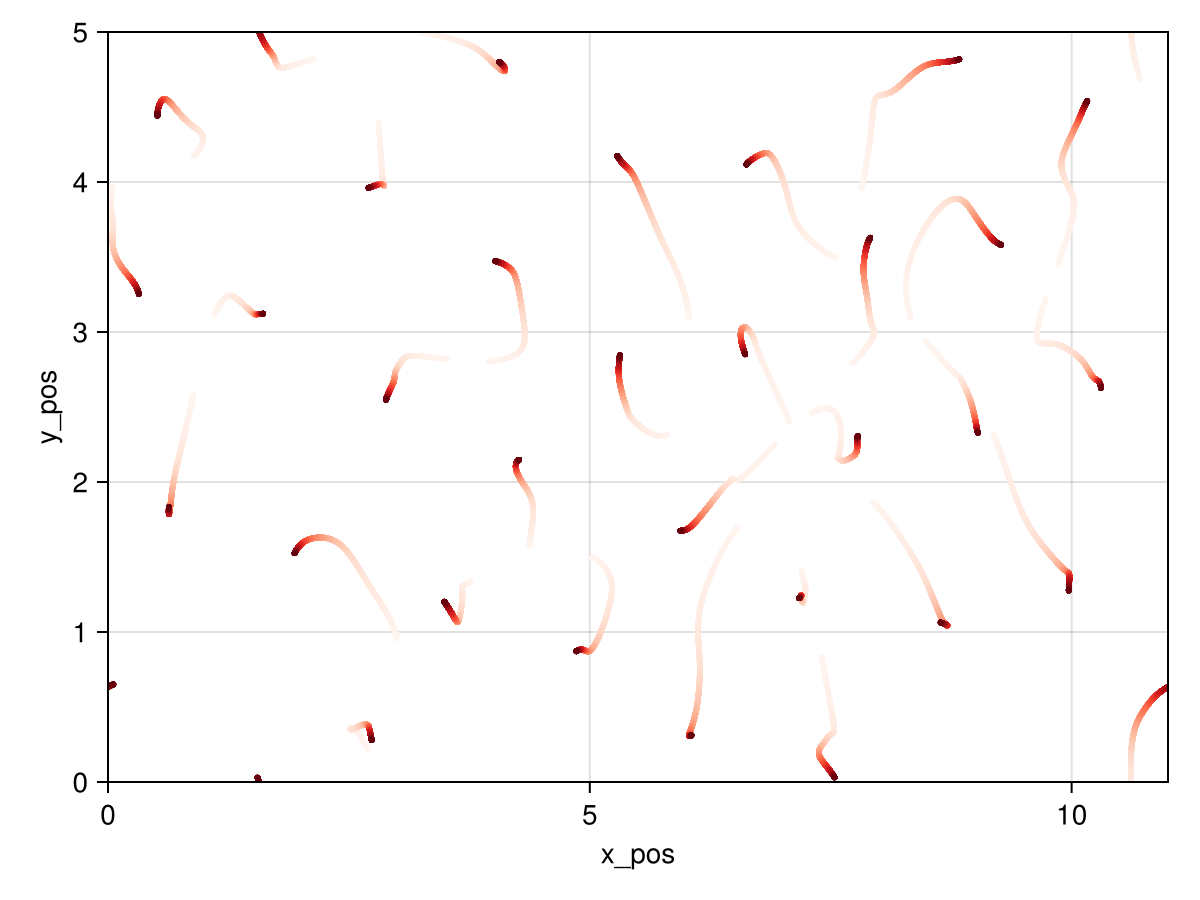
\includegraphics[width=0.6\linewidth]{figures/crystallizationdflow_4001.png}
        \caption{Pedestrian trajectories}
        \label{plot:crys_traj}
    \end{subfigure}
    \begin{subfigure}{.40\textwidth}
        \centering
        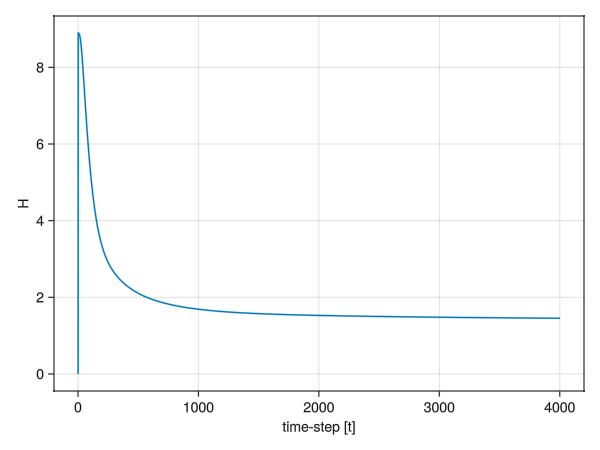
\includegraphics[width=\linewidth]{figures/H_crystallization.png}
        \caption{Hamiltonian $(H)$}
        \label{plot:crys_h}
    \end{subfigure}
    \begin{subfigure}{.40\textwidth}
        \centering
        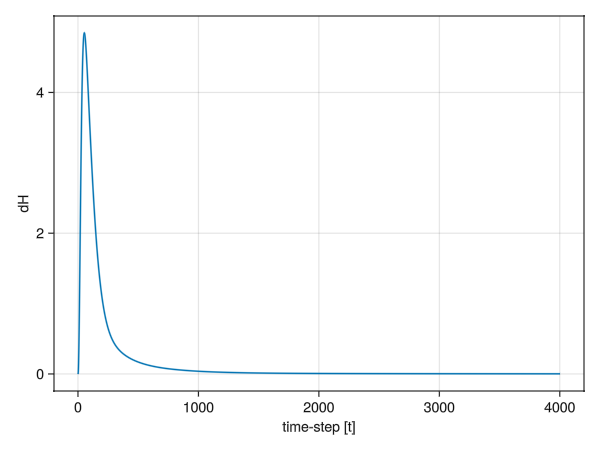
\includegraphics[width=\linewidth]{figures/dH_crystallization.png}
        \caption{Time derivative of Hamiltonian $\frac{d}{dt}H$}
        \label{plot:crys_dh}
    \end{subfigure}
    \caption{Crystallization of pedestrians due to no input $u_i = 0$ and allowing the system to dissipate energy}
    \label{plot:crys}
\end{figure}
Allowing the system to dissipate $\lambda > 0$ while simultaneously the pedestrians have no desired velocity \autoref{plot:crys}, essentially creates a system with an active output port, but no input. The results are as expected, the system keeps losing energy leading the pedestrians to crystallize over time. The Hamiltonian, which is a representation of the total energy of the system relaxes towards lower energy levels asymptotically reaching zero.
\pagebreak
\item \textbf{No dissipation ($\lambda = 0$)}
\begin{figure}[H]
    \centering
    \begin{subfigure}{\textwidth}
        \centering
        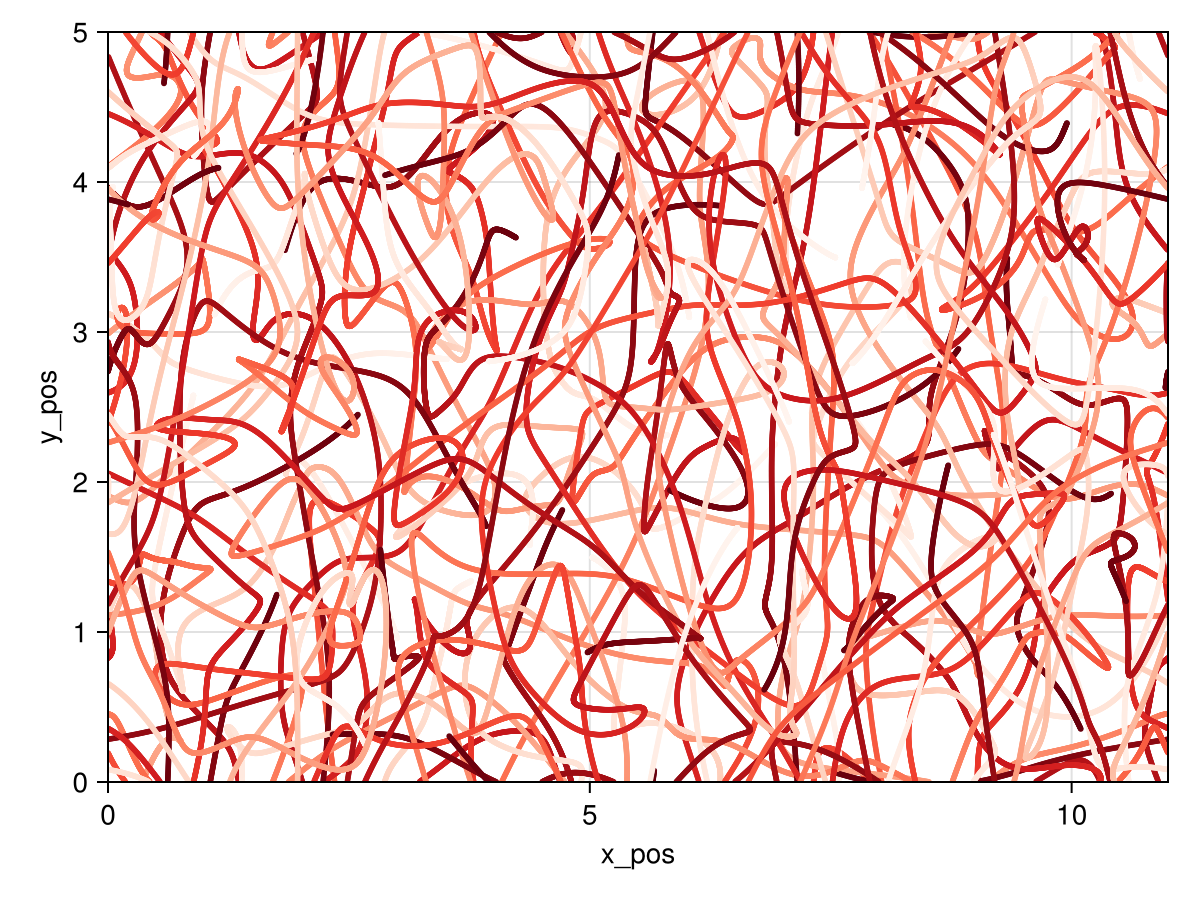
\includegraphics[width=0.6\linewidth]{figures/no_dissipationdflow_4001.png}
        \caption{Pedestrian trajectories}
        \label{plot:nodisp_traj}
    \end{subfigure}
    \begin{subfigure}{.40\textwidth}
        \centering
        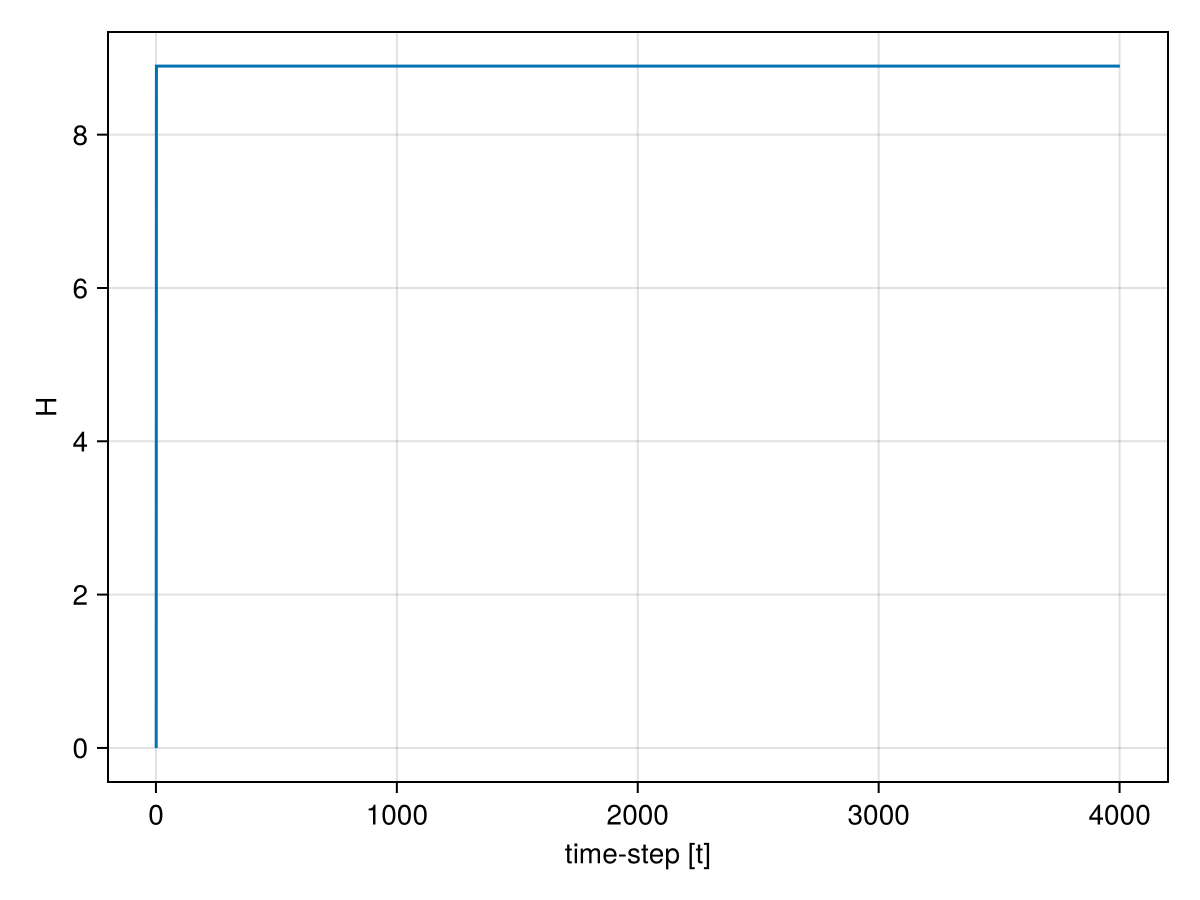
\includegraphics[width=\linewidth]{figures/H_no_dissipation.png}
        \caption{Hamiltonian $(H)$}
        \label{plot:nodisp_h}
    \end{subfigure}
    \begin{subfigure}{.40\textwidth}
        \centering
        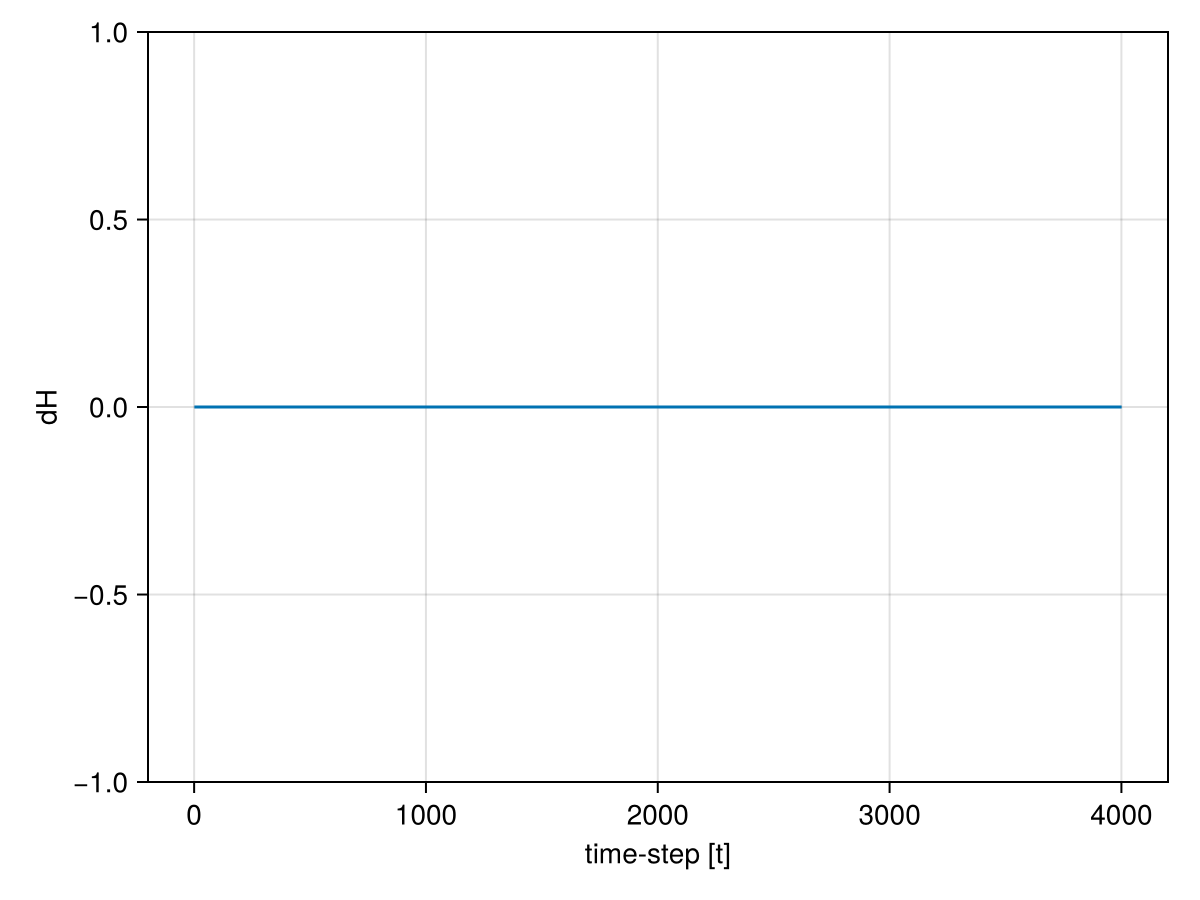
\includegraphics[width=\linewidth]{figures/dH_no_dissipation.png}
        \caption{Time derivative of Hamiltonian $\frac{d}{dt}H$}
        \label{plot:nodisp_dh}
    \end{subfigure}
    \caption{Trajectories of pedestrians in a non-dissipative system ($\lambda = 0$)}
    \label{plot:nodisp}
\end{figure}

Given the dynamics formulated in \autoref{eq:ph_model}, it can be clearly seen that $\lambda$ exists both as a coefficient of the input port $\tilde u$ as well as in the output port $y$. Thus setting $\lambda = 0$ clearly suggests that the resulting system has no dissipation as well as no energy feed. Consequently, the pedestrians move with no direction \autoref{plot:nodisp_traj} regardless of the fact the desired velocity is provided.

The resulting system is a conservative Hamiltonian system, as by consequence the dissipative term $R$ also vanishes. This can be clearly observed as the Hamiltonian remains constant over time. It is to be noted that the immediate jump of the Hamiltonian in \autoref{plot:nodisp_h} is simply because the Hamiltonian was initialized to zero (\autoref{code:model_init}) before the start of the simulation
\pagebreak
\item \textbf{No pedestrian interaction ($A = 0$) with $u_i = \begin{bmatrix} 1 & 0 \end{bmatrix}$}
\begin{figure}[H]
    \centering
    \begin{subfigure}{\textwidth}
        \centering
        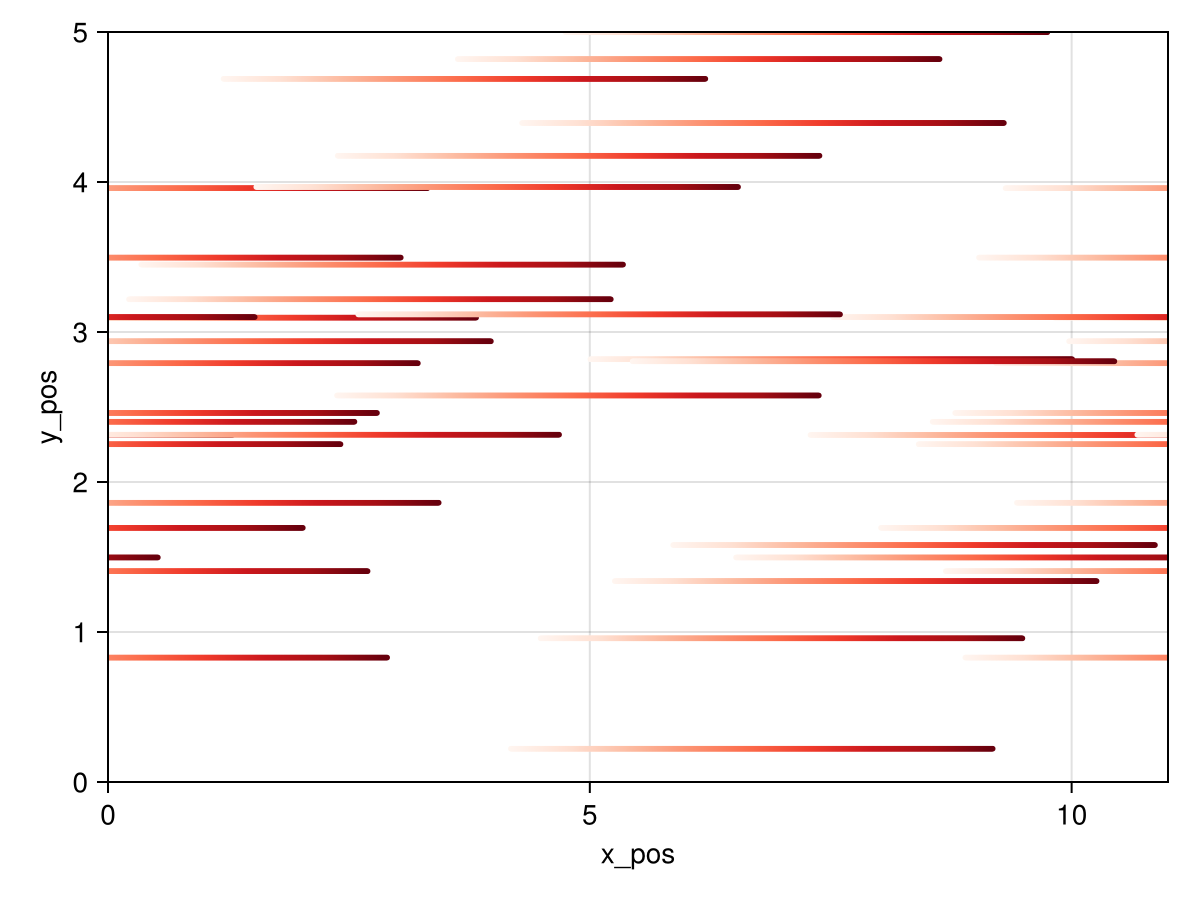
\includegraphics[width=0.6\linewidth]{figures/no_interactiondflow_4000.png}
        \caption{Pedestrian trajectories}
        \label{plot:nointeraction_traj}
    \end{subfigure}
    \begin{subfigure}{.40\textwidth}
        \centering
        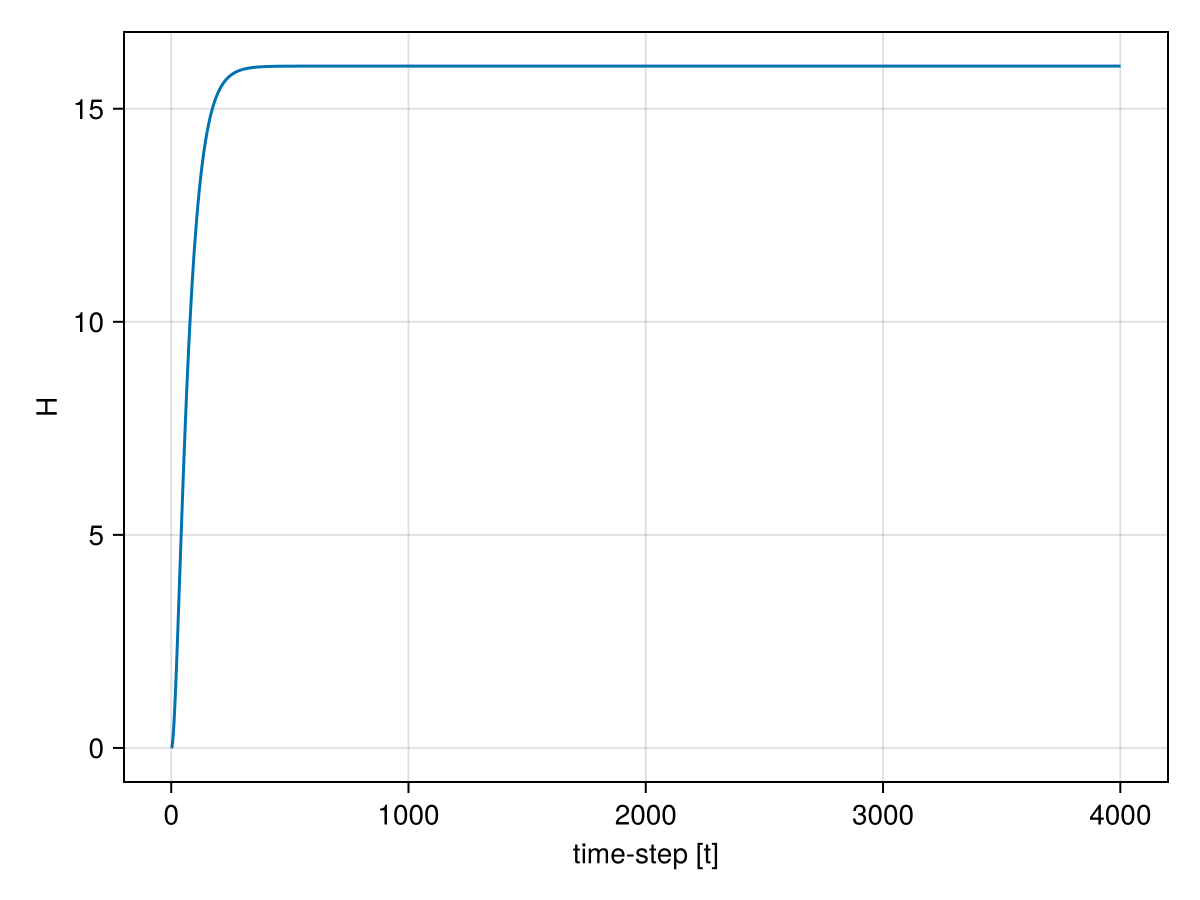
\includegraphics[width=\linewidth]{figures/H_no_interaction.png}
        \caption{Hamiltonian $(H)$}
        \label{plot:nointeraction_h}
    \end{subfigure}
    \begin{subfigure}{.40\textwidth}
        \centering
        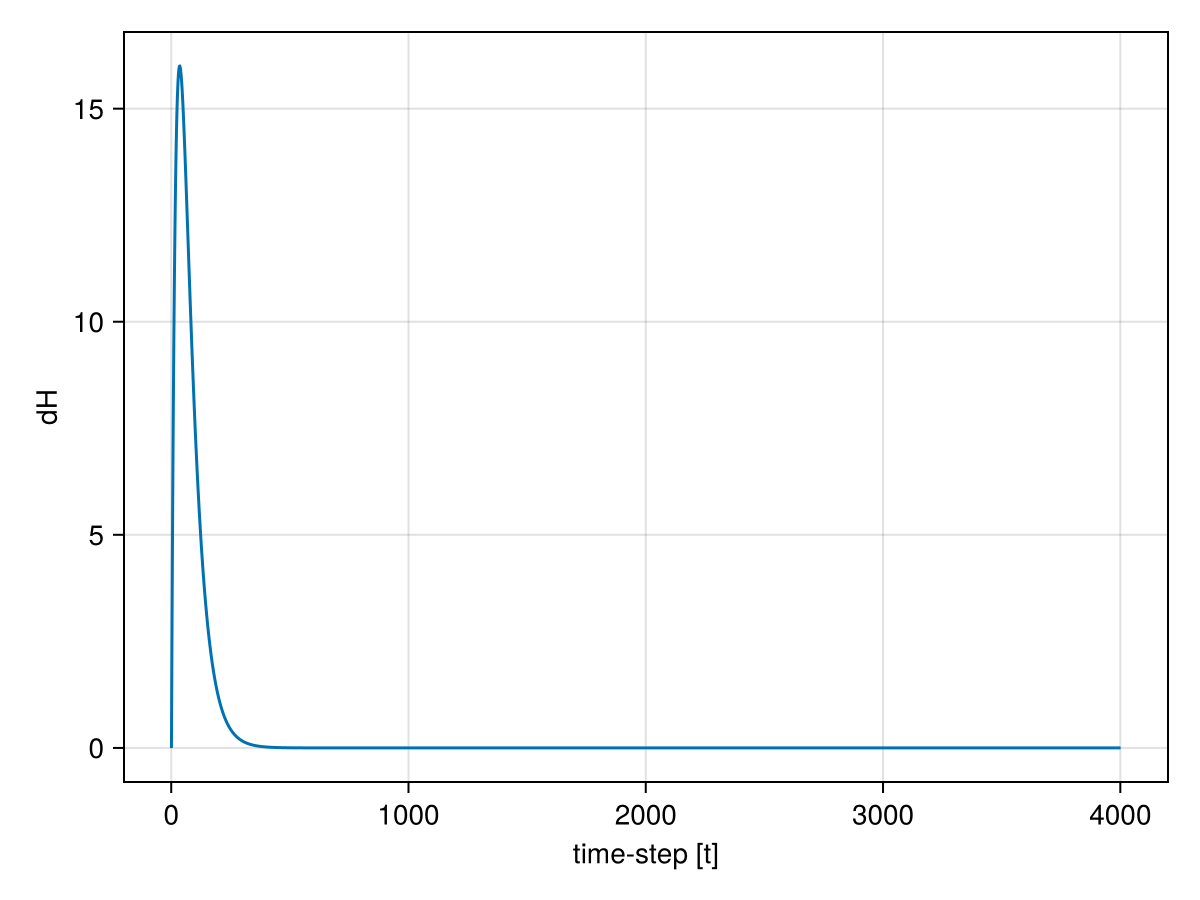
\includegraphics[width=\linewidth]{figures/dH_no_interaction.png}
        \caption{Time derivative of Hamiltonian $\frac{d}{dt}H$}
        \label{plot:nointeraction_dh}
    \end{subfigure}
    \caption{Trajectories of pedestrians with no interaction with other pedestrian ($ A = 0 $) and desired velocities $u_i = \begin{bmatrix}1 & 0\end{bmatrix} $}
    \label{plot:nointeraction}
\end{figure}

By setting $A = 0$, the pedestrians in the system move with no interactivity with other pedestrians in the system. Essentially, every pedestrian simply move with their desired velocities as soon the simulation begins \autoref{plot:nointeraction}. Because this parameter directly effects the interaction potential $U(x)$ in \autoref{eq:def_potU}, it can be clearly observed that the motion of the pedestrian is independent of their distance to each other, in other words they move with no concern to how close or far they are from other pedestrians.

Given the lack of interaction, the pedestrians move with their desired velocities, thus in the long run, the Hamiltonian need not be dependent on time, but instead the desired velocities of the pedestrians -- mathematically $p_i = u_i$. One can also obtain this long term value of the Hamiltonian $H^*(u)$ by setting $A = 0$ (as it is for this case) in \autoref{eq:Hamiltonian} leading to 
\begin{align}
    H(z(t)) = \dfrac{1}{2}||p(t)||^2 \rightarrow H^*(u) = \dfrac{1}{2}||u||^2
    \label{eq:Hstar}
\end{align}

This expression for the long term Hamiltonian $H^*(u)$ is a function of the desired velocities $u_i$. As $u_i$ is set by the user, one easily evaluate this value. Even with potential interaction allowed in the system dynamics, the expression serves as a representation of what the system as a whole is trying to attain. Ideally, every pedestrian wants to achieve the desired velocity $u_i$, and the system as a whole wants to achieve the energy $H^*$. 
\end{itemize}



\subsection{Collective Dynamics}
\label{section:collective}

In this section however, we will witness collective phenomenon based on the desired speeds and relaxation (or dissipation) parameter $\lambda$. The pedestrians will start from the same random positions generated in \autoref{plot:starting_pos}, but with different desired speeds $u_i$. This disordered arrangement goes through a phase transition and form ordered patterns, such as lane formation and stripe formation. We will notice how a sufficient $\lambda$ is needed to achieve these phase transitions. Furthermore, we will see how $H^*(u)$ from \autoref{eq:Hstar} ties in as an order parameter to identify collective behaviors.
\begin{itemize}
    \item \textbf{Lane Formation for counter flow with $\lambda = 2$}
    \begin{figure}[H]
        \centering
        \begin{subfigure}{\textwidth}
            \centering
            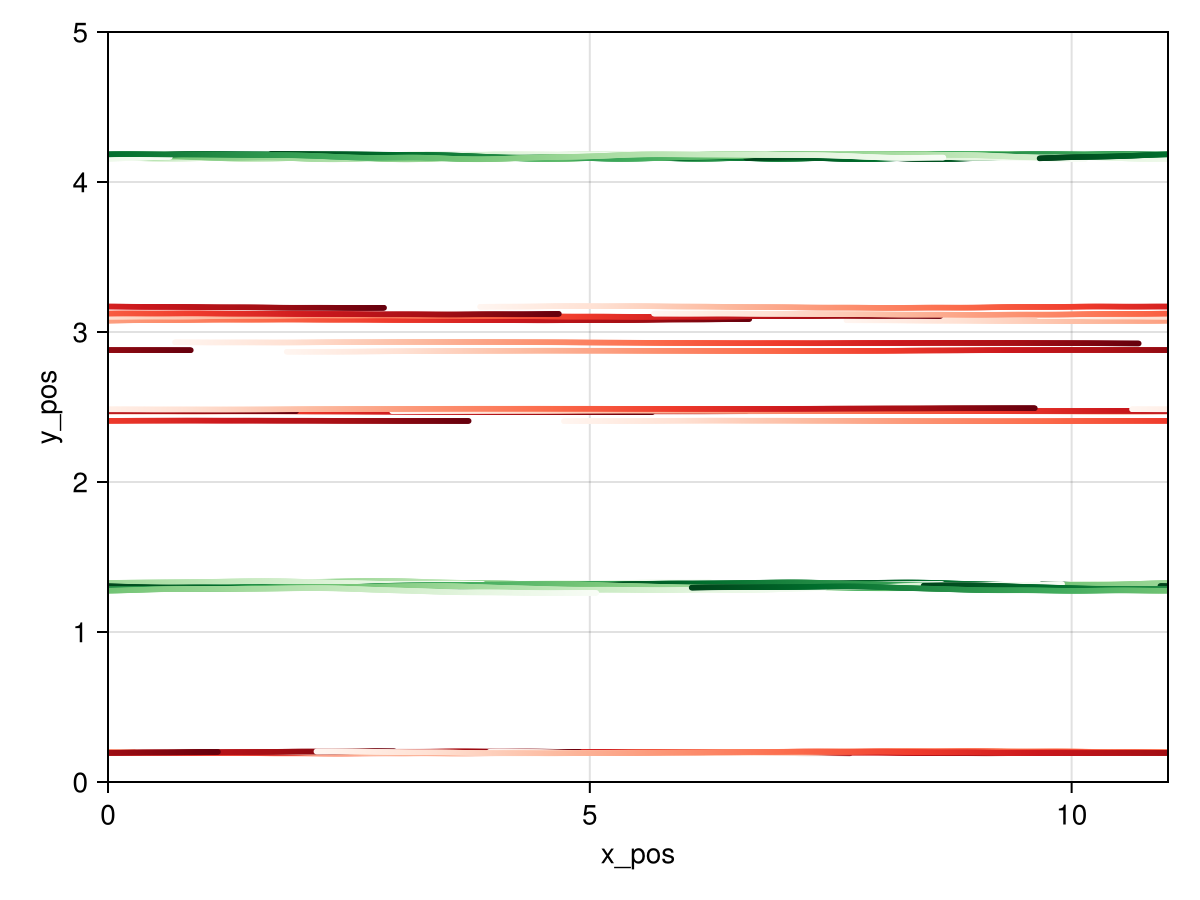
\includegraphics[width=0.6\linewidth]{figures/s0_fbh_1noflow_10000.png}
            \caption{Pedestrian trajectories}
            \label{plot:counter_traj}
        \end{subfigure}
        \begin{subfigure}{.40\textwidth}
            \centering
            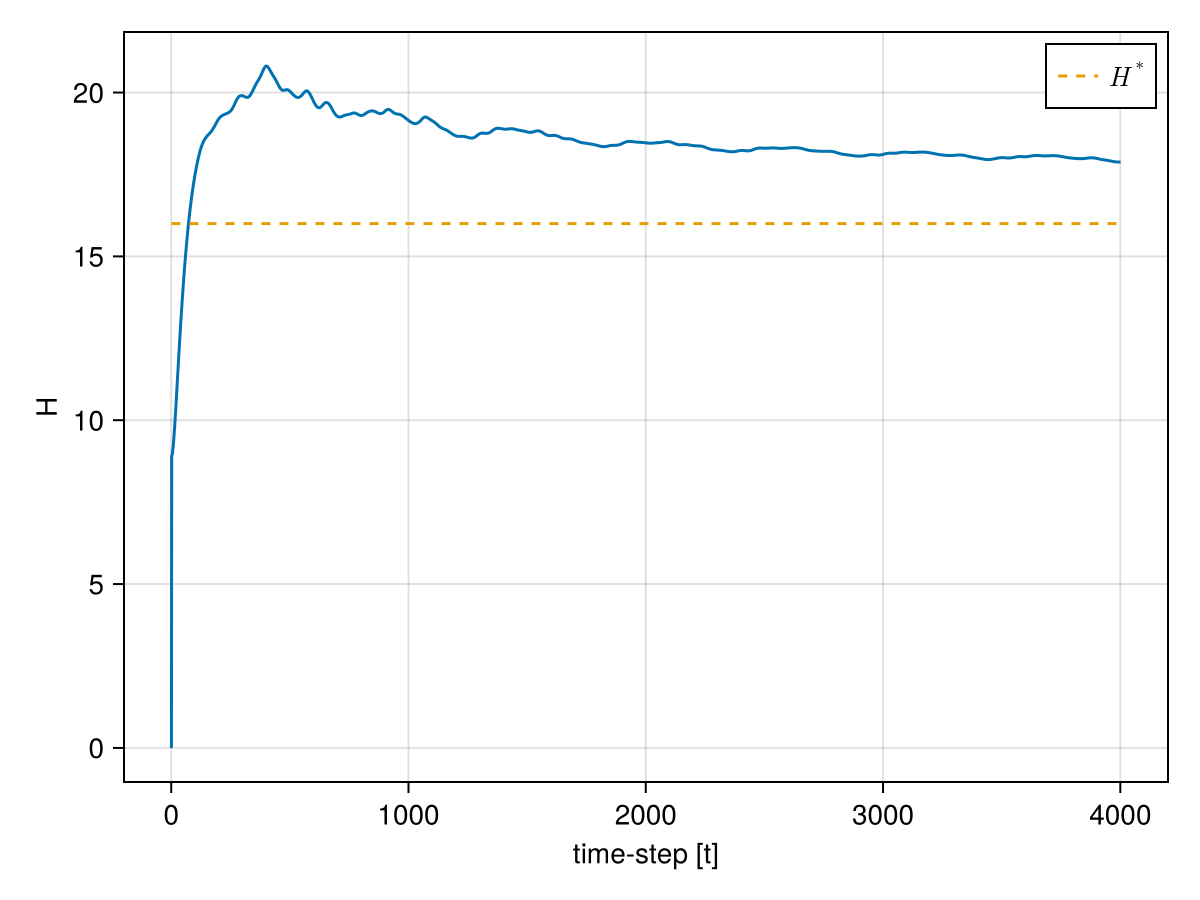
\includegraphics[width=\linewidth]{figures/H_counter.png}
            \caption{Hamiltonian $(H)$}
            \label{plot:counter_h}
        \end{subfigure}
        \begin{subfigure}{.40\textwidth}
            \centering
            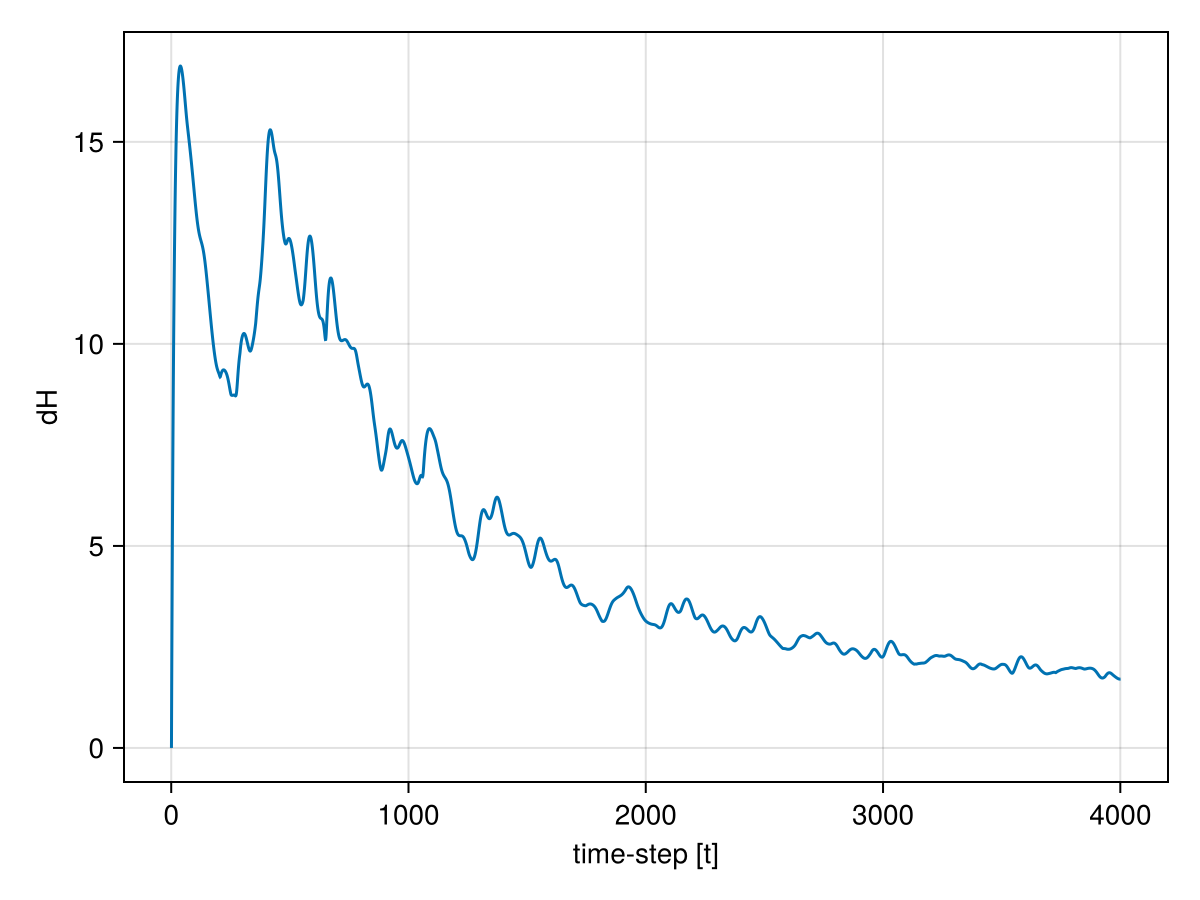
\includegraphics[width=\linewidth]{figures/dH_counter.png}
            \caption{Time derivative of Hamiltonian $\frac{d}{dt}H$}
            \label{plot:counter_dh}
        \end{subfigure}
        \caption{Emergence of lane formation as pedestrians move in counter flow}
        \label{plot:counter}
    \end{figure}
Starting from a random assortment of pedestrians as shown in \autoref{plot:starting_pos}, with predefined desired velocities $u_i = \begin{bmatrix} 1 & 0 \end{bmatrix}$ for half of the pedestrians (Red), and $u_i = \begin{bmatrix} -1 & 0 \end{bmatrix}$ for the other half (Green), as shown in \autoref{code:agent_init}. As the time progresses, the pedestrians form lanes. From a point of view of energy in the system, the pedestrians self-organize themselves in a manner such that the Hamiltonian reaches a steady state and remains above $H^*$, while $\frac{d}{dt}H$ reaches zero. 

    \item \textbf{Gridlock for counter flow with $\lambda = 0.2$}
    \begin{figure}[H]
        \centering
        \begin{subfigure}{\textwidth}
            \centering
            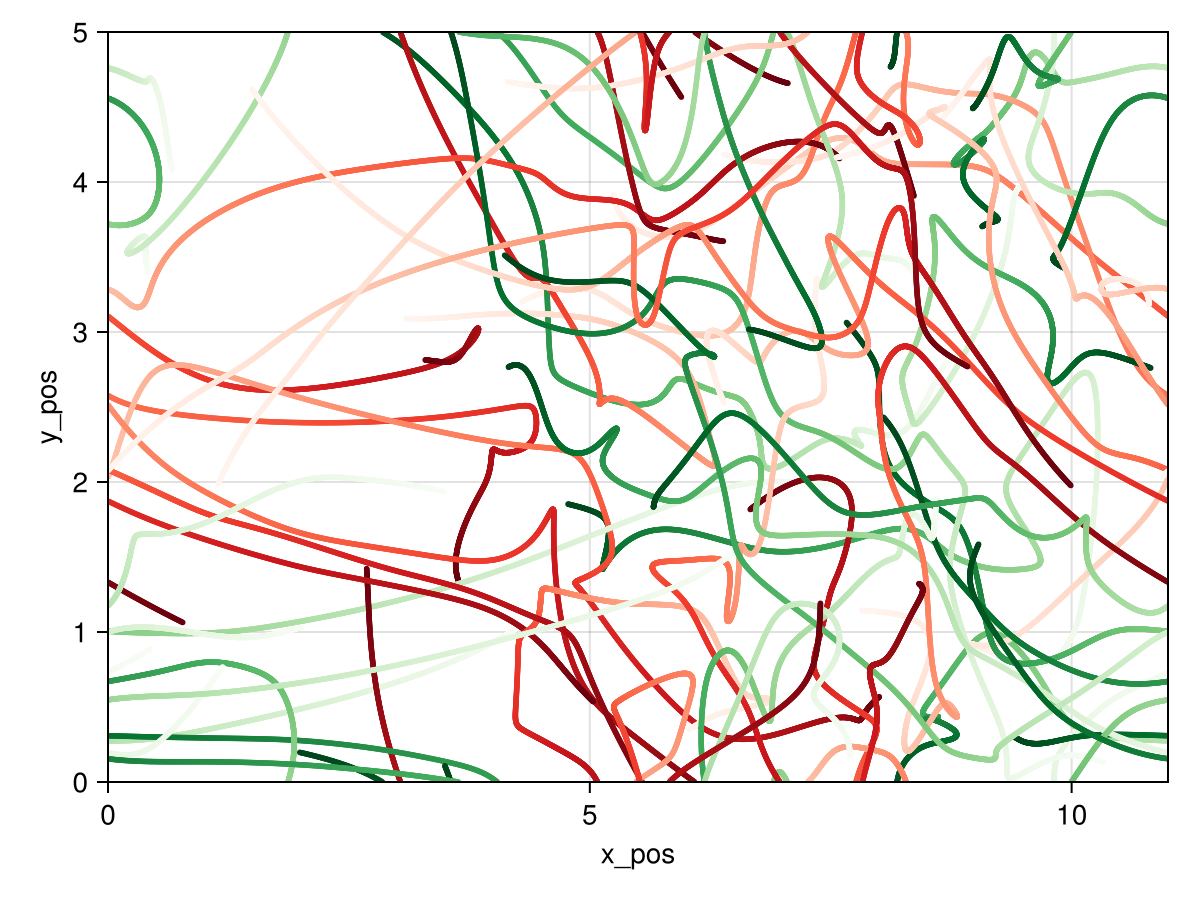
\includegraphics[width=0.6\linewidth]{figures/counter_gridlockdflow_4000.png}
            \caption{Pedestrian trajectories}
            \label{plot:countergridlock_traj}
        \end{subfigure}
        \begin{subfigure}{.40\textwidth}
            \centering
            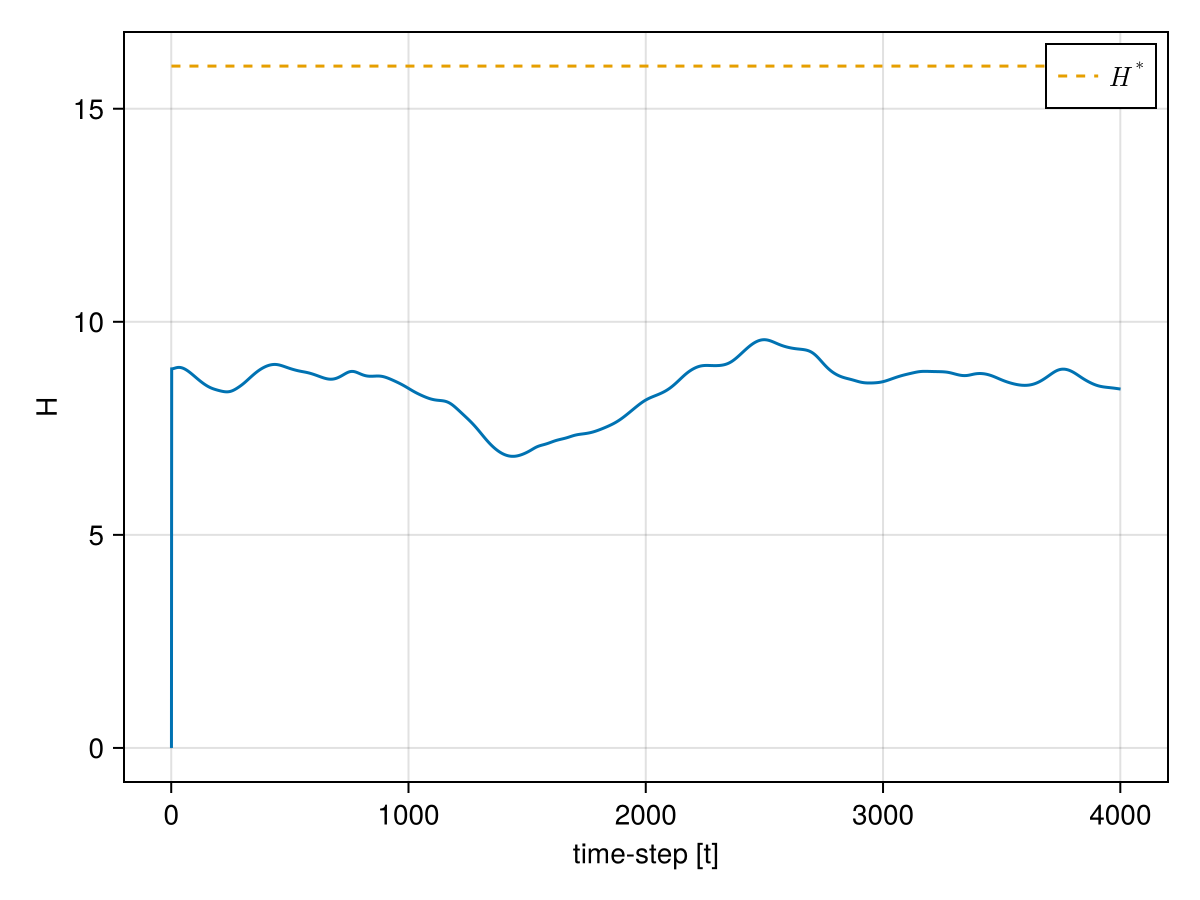
\includegraphics[width=\linewidth]{figures/H_counter_gridlock.png}
            \caption{Hamiltonian $(H)$}
            \label{plot:countergridlock_h}
        \end{subfigure}
        \begin{subfigure}{.40\textwidth}
            \centering
            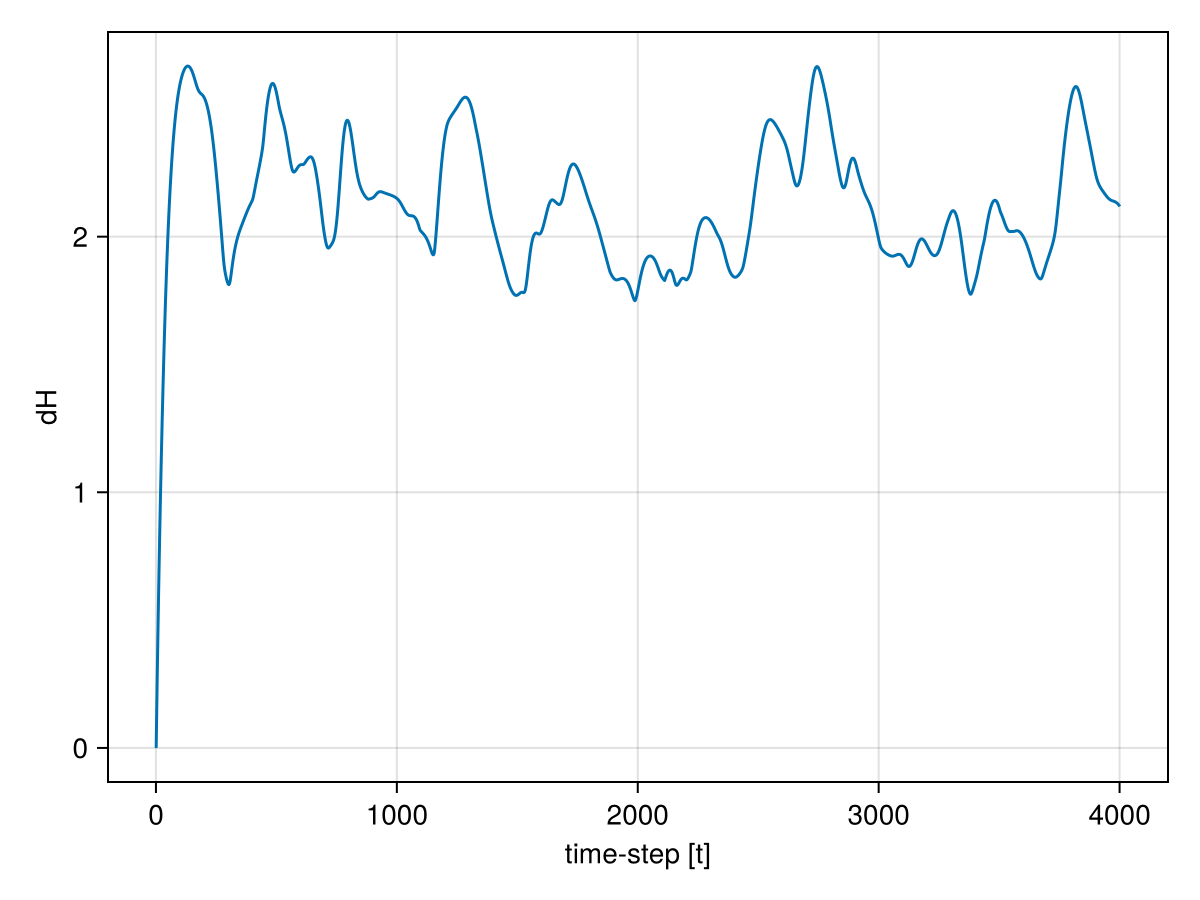
\includegraphics[width=\linewidth]{figures/dH_counter_gridlock.png}
            \caption{Time derivative of Hamiltonian $\frac{d}{dt}H$}
            \label{plot:countergridlock_dh}
        \end{subfigure}
        \caption{Gridlock for counter flow}
        \label{plot:countergridlock}
    \end{figure}
With the same parameters as the previous case, with the only difference being that $\lambda$ is not sufficiently high, it can be observed that no lane formation occurs. The system neither gains nor dissipates enough energy, resulting in pedestrians behaving similarly to the trajectories presented in \autoref{plot:nodisp}, leading to gridlocks. The Hamiltonian erratically fluctuates over time and remains below $H^*$.

Here the significance of $\lambda$ is apparent, as this parameter balances the conservation of energy enforced by the skew-symmetry with the flow of energy through dissipation and feed permitted by the ports.
\pagebreak
    \item \textbf{Stripe Formation for cross flow with $\lambda = 2$}
    \begin{figure}[H]
        \centering
        \begin{subfigure}{\textwidth}
            \centering
            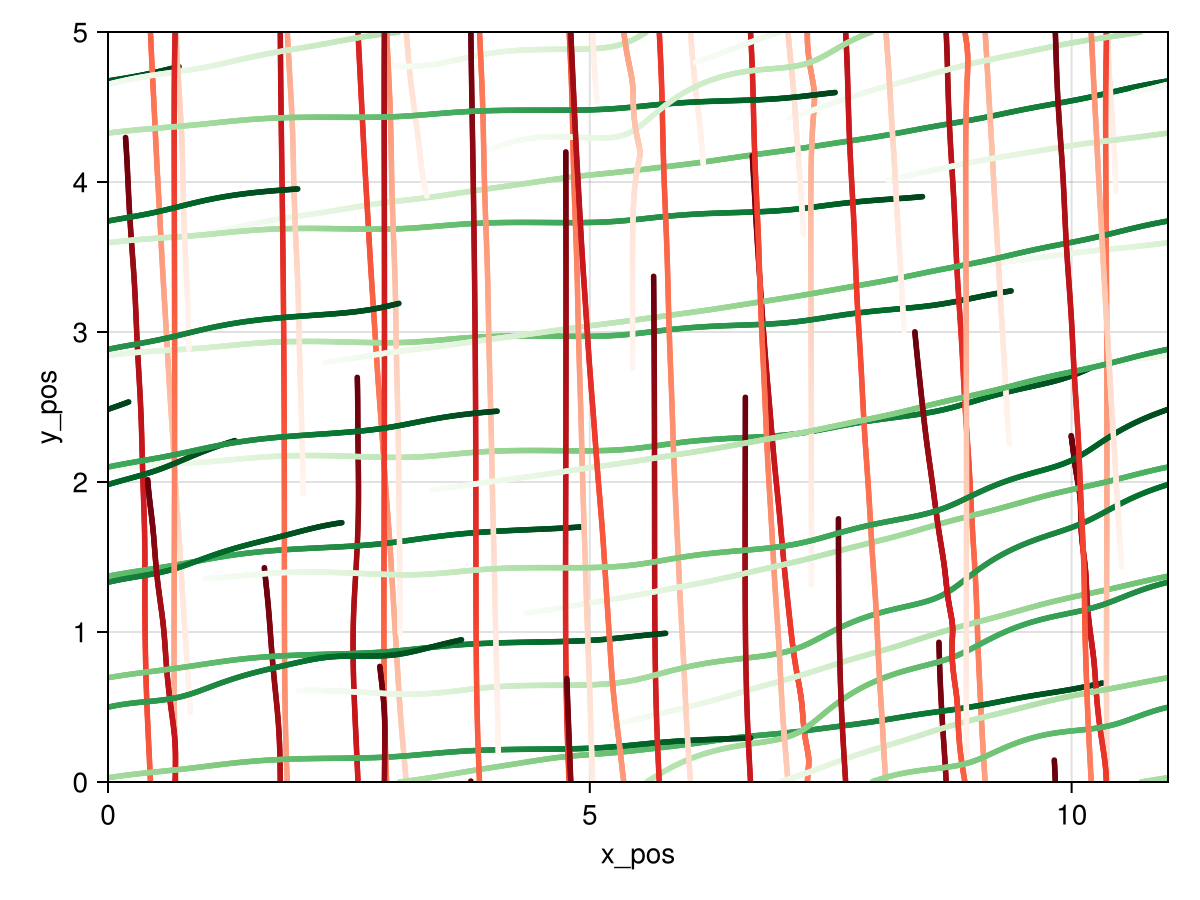
\includegraphics[width=0.6\linewidth]{figures/crossleapflow_10000.png}
            \caption{Pedestrian trajectories}
            \label{plot:cross2_traj}
        \end{subfigure}
        \begin{subfigure}{.40\textwidth}
            \centering
            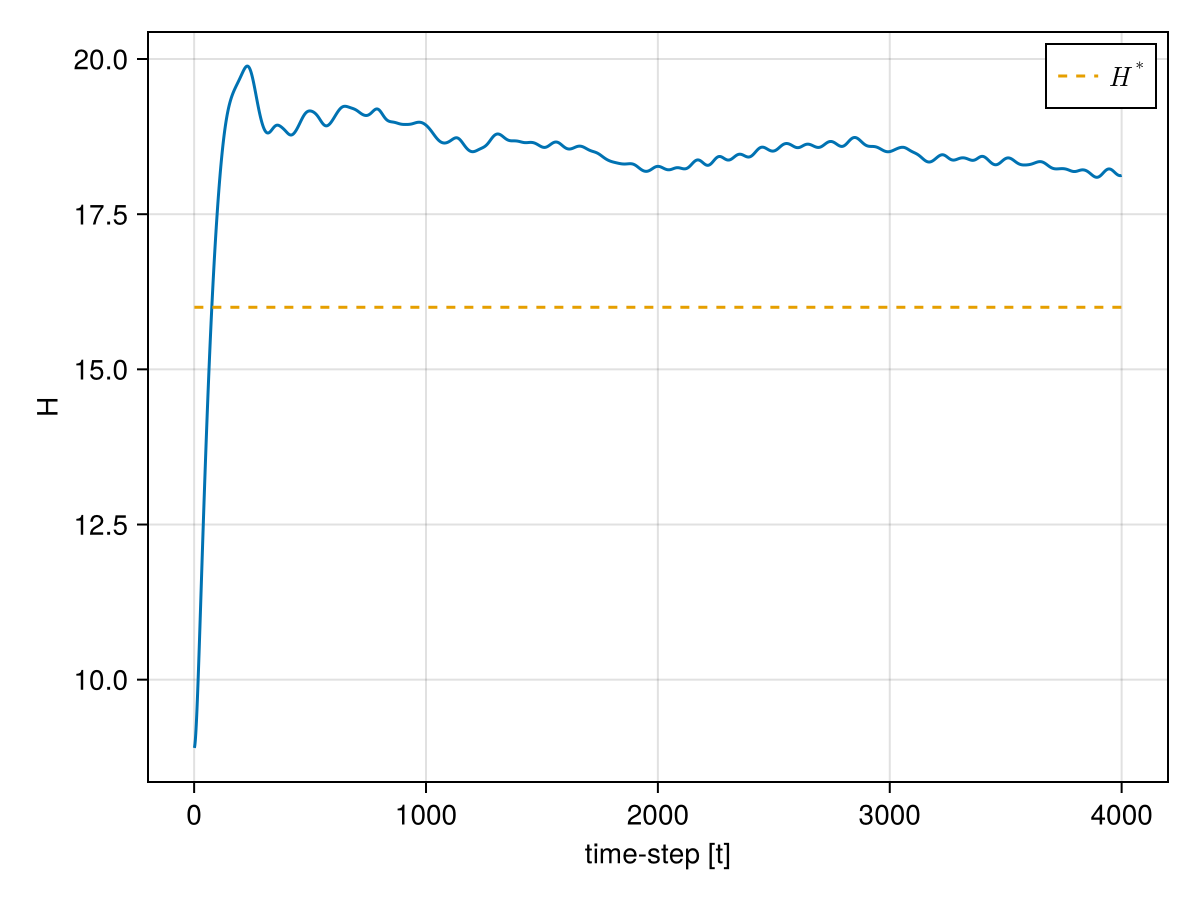
\includegraphics[width=\linewidth]{figures/H_cross2.png}
            \caption{Hamiltonian $(H)$}
            \label{plot:cross2_h}
        \end{subfigure}
        \begin{subfigure}{.40\textwidth}
            \centering
            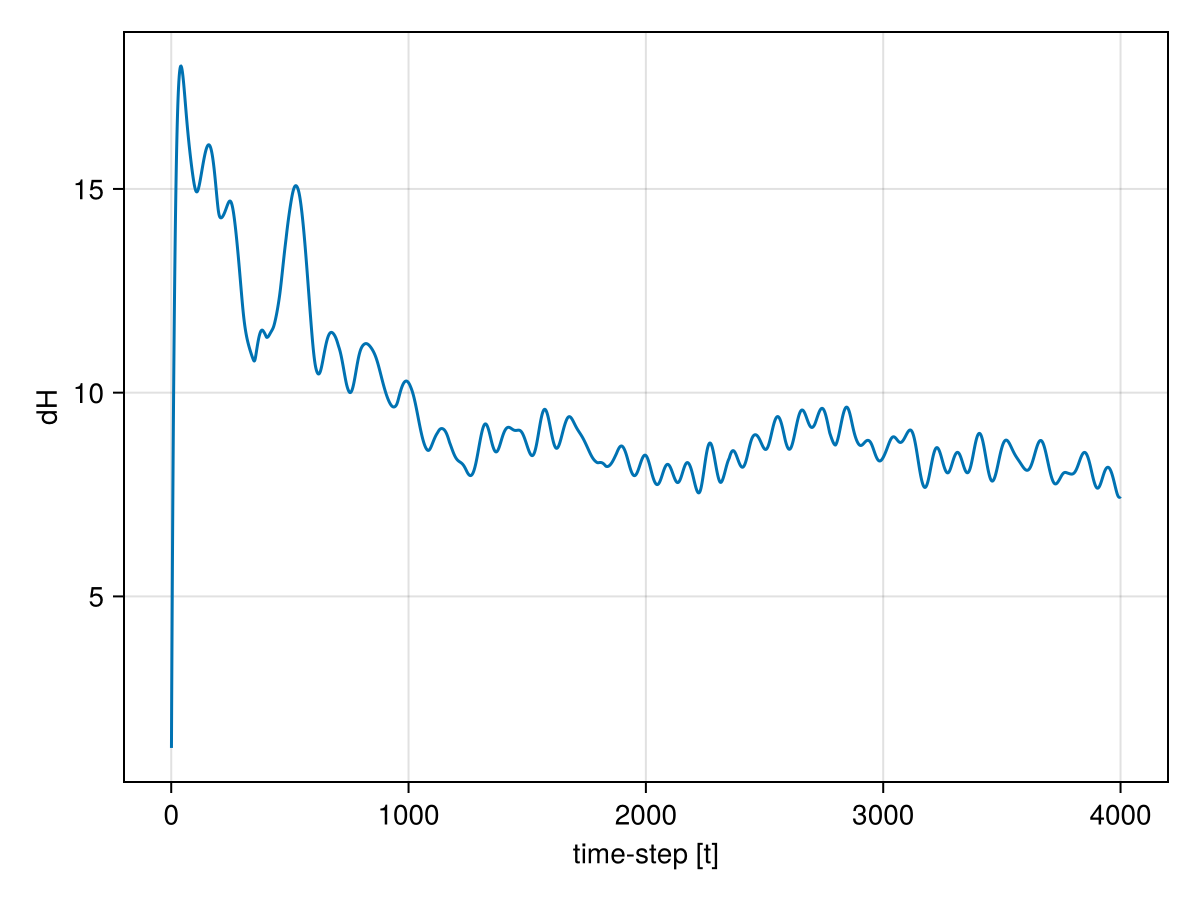
\includegraphics[width=\linewidth]{figures/dH_cross2.png}
            \caption{Time derivative of Hamiltonian $\frac{d}{dt}H$}
            \label{plot:cross2_dh}
        \end{subfigure}
        \caption{Stripe formation at a diagonal for cross flow with $\lambda = 2$}
        \label{plot:cross2}
    \end{figure}
Starting from the same positions as \autoref{plot:starting_pos} with the desired velocities set to $u_i = \begin{bmatrix} 1 & 0 \end{bmatrix}$ for half of the pedestrians (Green), and $u_i = \begin{bmatrix} 0 & 1 \end{bmatrix}$ for the other half (Red). We can observe that the pedestrians form a \textit{diagonal} stripe formation; they are not able to reach the desired direction with much ease, forming an angled trajectory. This is also apparent when we look at the plots for the Hamiltonian, as the $\frac{d}{dt}H$ fluctuates over time. However, the long term dynamics of the pedestrians would result in an arrangement where the pedestrians don't deviate from their desired directions, as shown in the next case.

\pagebreak
    \item \textbf{Stripe Formation for cross flow with $\lambda = 3$}
    \begin{figure}[H]
        \centering
        \begin{subfigure}{\textwidth}
            \centering
            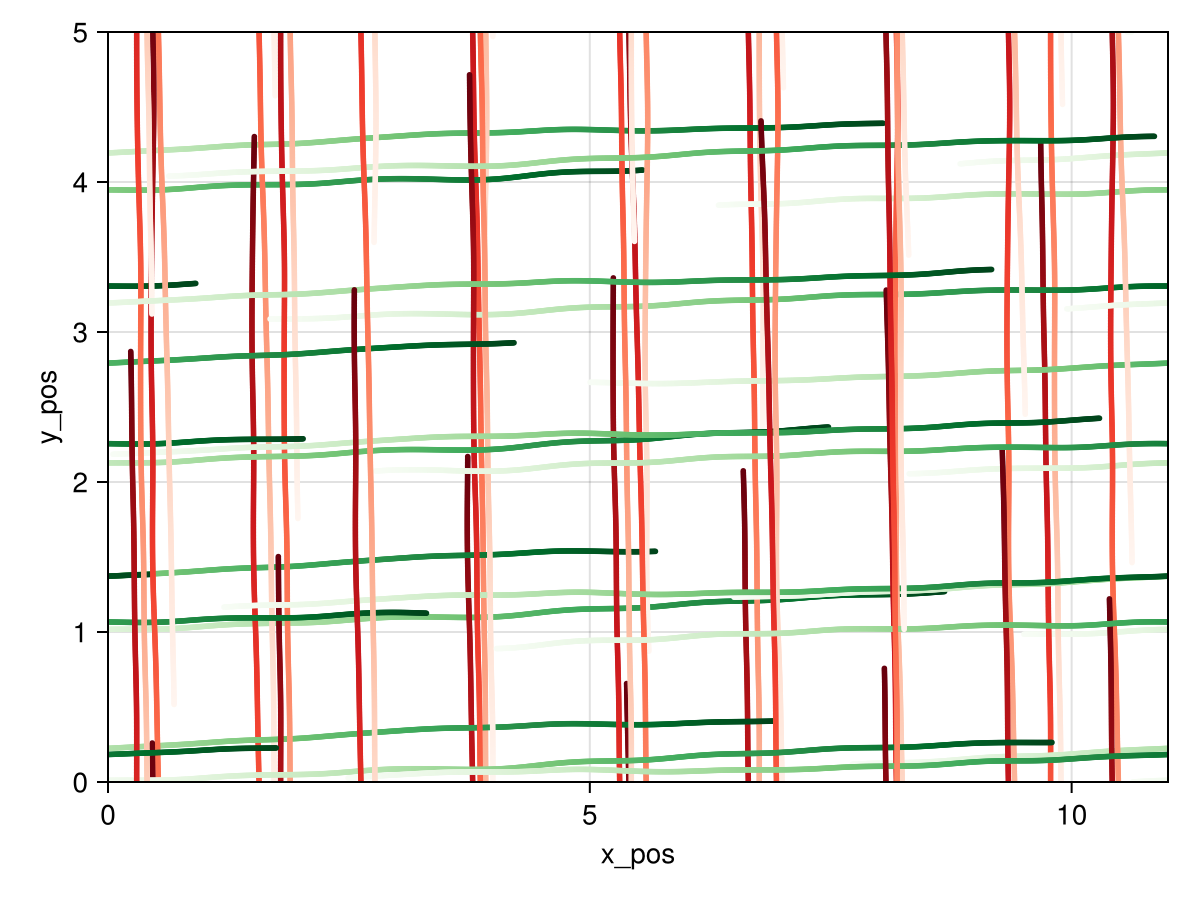
\includegraphics[width=0.6\linewidth]{figures/s0crossleap3flow_10000.png}
            \caption{Pedestrian trajectories}
            \label{plot:cross_traj}
        \end{subfigure}
        \begin{subfigure}{.40\textwidth}
            \centering
            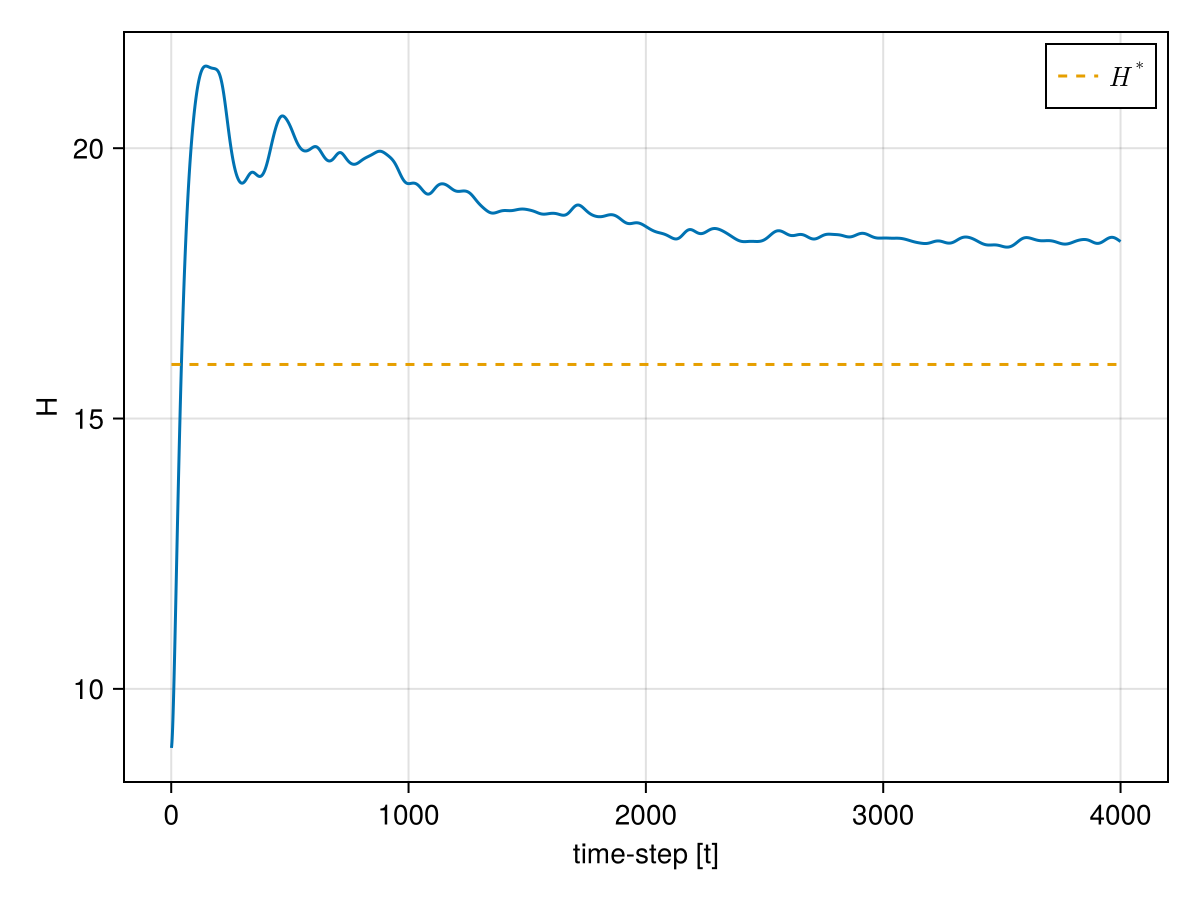
\includegraphics[width=\linewidth]{figures/H_cross.png}
            \caption{Hamiltonian $(H)$}
            \label{plot:cross_h}
        \end{subfigure}
        \begin{subfigure}{.40\textwidth}
            \centering
            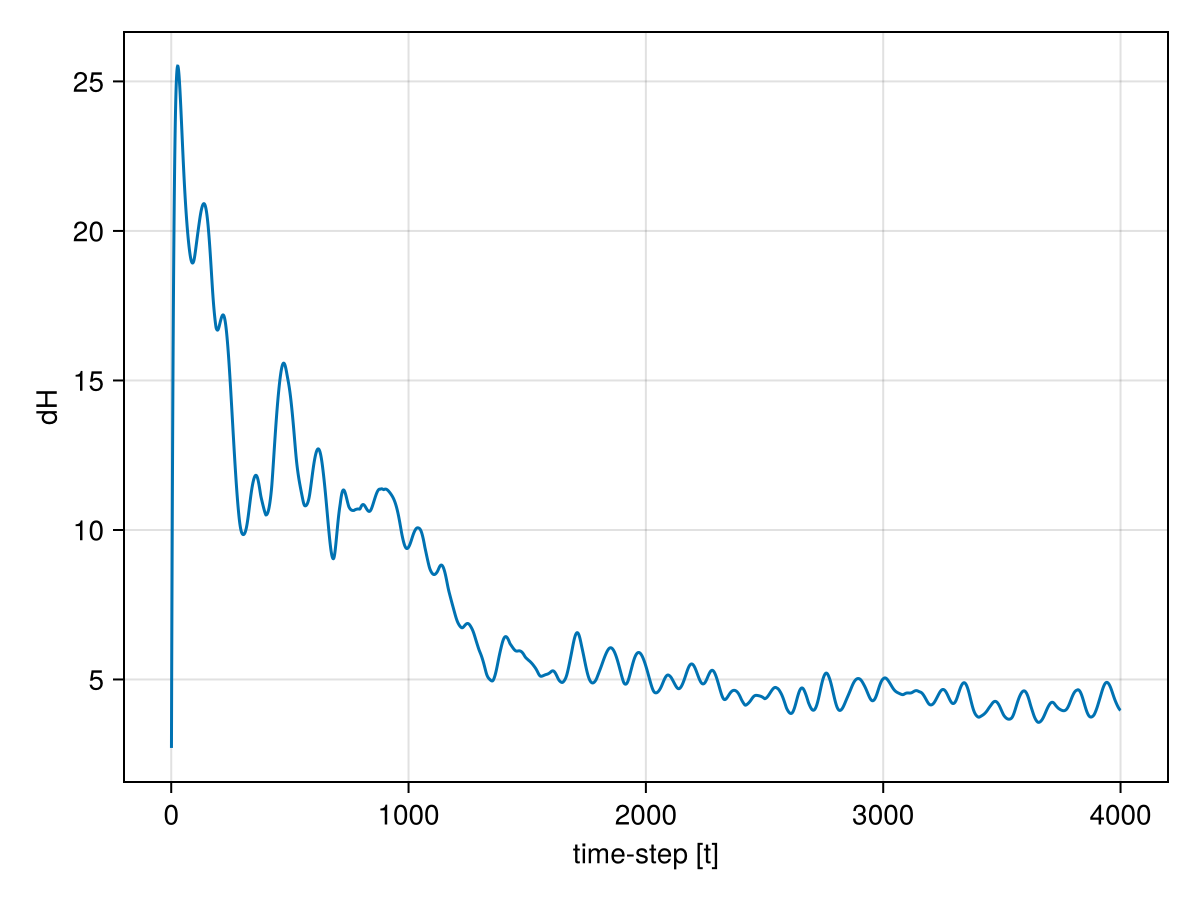
\includegraphics[width=\linewidth]{figures/dH_cross.png}
            \caption{Time derivative of Hamiltonian $\frac{d}{dt}H$}
            \label{plot:cross_dh}
        \end{subfigure}
        \caption{Stripe formation for cross flow with $\lambda = 3$}
        \label{plot:cross3}
    \end{figure}
Here we replicate the model from before, though we set $\lambda$ to a higher value, we can clearly observe a better stripe formation. The Hamiltonian also doesn't fluctuate too much as $\frac{d}{dt}H$ decreases more quickly. In both of these cases, we can observe that the stripe formation occurs, and the Hamiltonian remains above $H^*$
\pagebreak    
    \item \textbf{Gridlock for cross flow with $\lambda = 0.2$}
    \begin{figure}[H]
        \centering
        \begin{subfigure}{\textwidth}
            \centering
            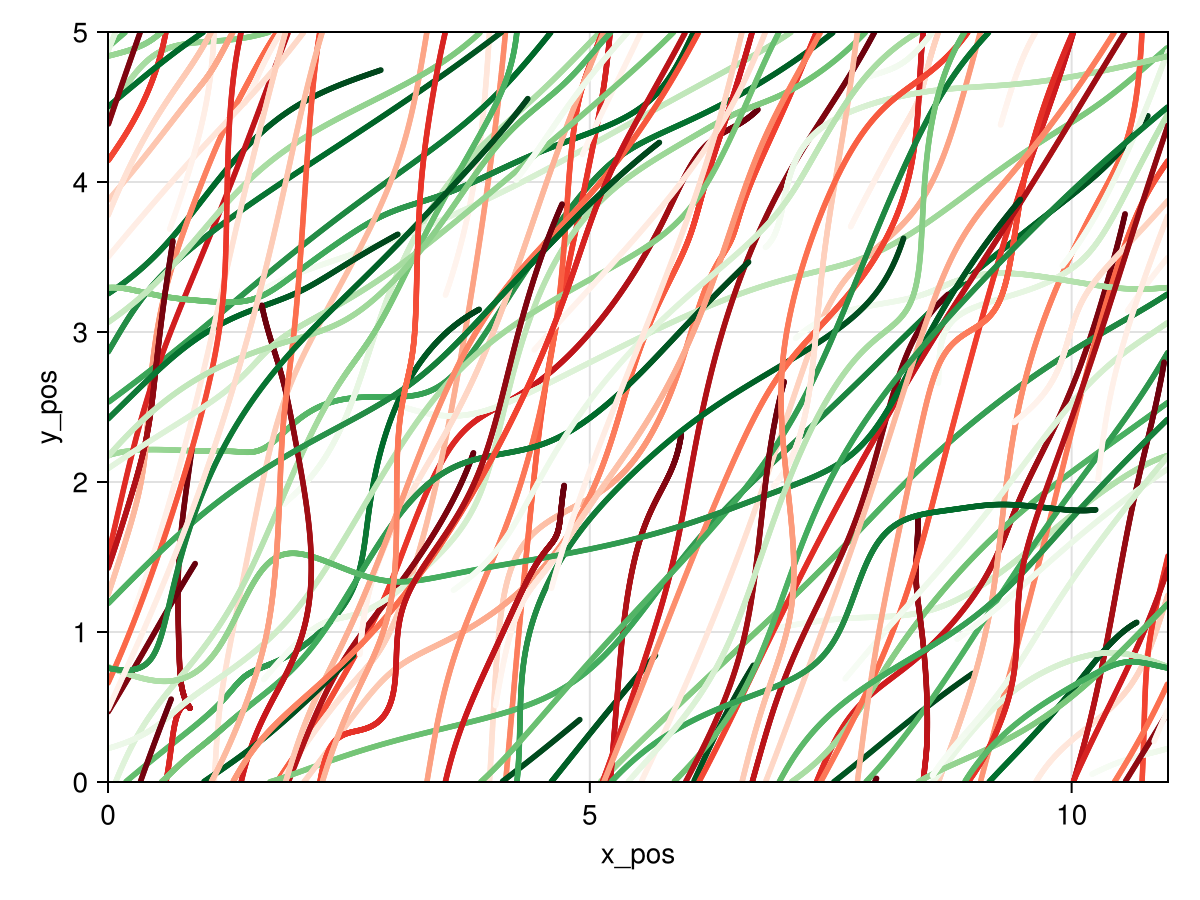
\includegraphics[width=0.6\linewidth]{figures/cross_gridlockdflow_4000.png}
            \caption{Pedestrian trajectories}
            \label{plot:crossgridlock_traj}
        \end{subfigure}
        \begin{subfigure}{.40\textwidth}
            \centering
            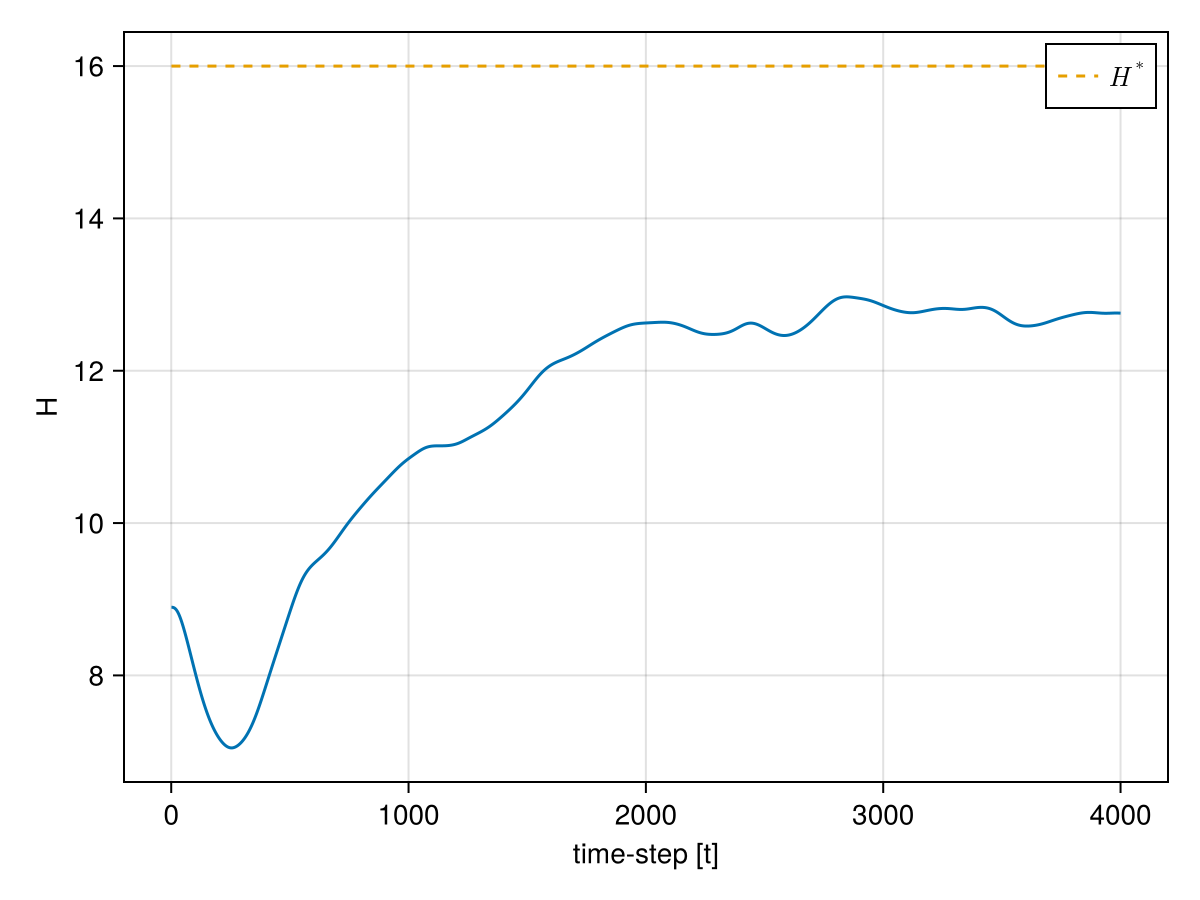
\includegraphics[width=\linewidth]{figures/H_cross_gridlock.png}
            \caption{Hamiltonian $(H)$}
            \label{plot:crossgridlock_h}
        \end{subfigure}
        \begin{subfigure}{.40\textwidth}
            \centering
            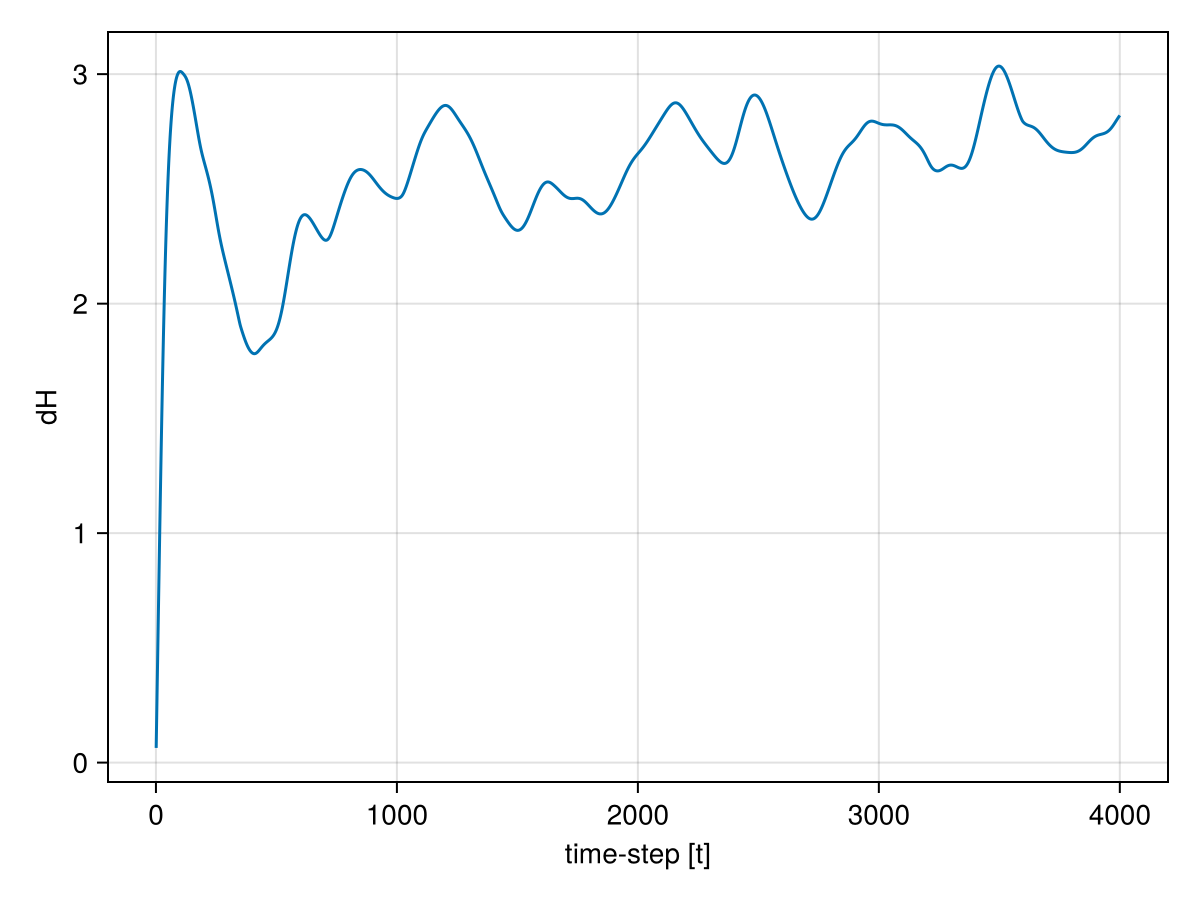
\includegraphics[width=\linewidth]{figures/dH_cross_gridlock.png}
            \caption{Time derivative of Hamiltonian $\frac{d}{dt}H$}
            \label{plot:crossgridlock_dh}
        \end{subfigure}
        \caption{Gridlock for cross flow}
        \label{plot:crossgridlock}
    \end{figure}
Here we can see that no stripe formation occurs, as $\lambda$ is not high enough for the pedestrians to be reactive. The Hamiltonian also remain below $H^*$
\end{itemize}

From the simulations above, we have observed that collective dynamics occur when the Hamiltonian remains above $H^*$. 
\pagebreak
\subsection{Stochastic Model Dynamics}
In this section, we once again pay our attention to the stochastic model dynamics. We will keep the same parameters as \autoref{code:model_init}, and focus mainly on three cases: unidirectional, counter, and cross flows. In all of these cases, we will increase the volatility $\sigma$ for every simulation. In a physical sense, one can interpret the addition of noise as 'warming' the system, and hence we will notice, for most cases, that the overall energy of the systems increase with increase in noise. We observe the long term dynamics and also the rate of change of Hamiltonian $\frac{d}{dt}H$ over time.

\begin{itemize}
    \item \textbf{Unidirectional flow ($\sigma \geq 0$)}
    \begin{figure}[H]
        \centering
        \begin{subfigure}{.49\textwidth}
            \centering
            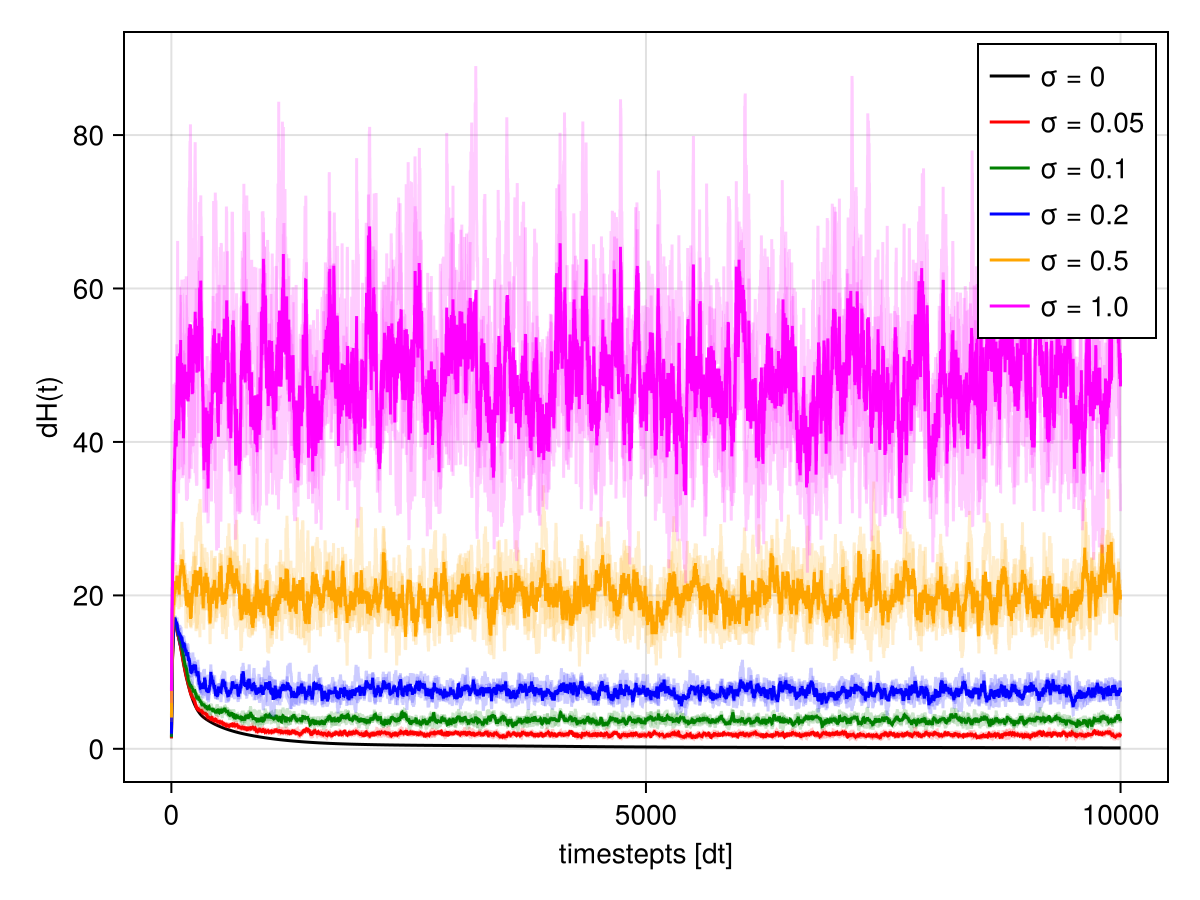
\includegraphics[width=\linewidth]{figures/dH_stochasic_uni.png}
            \caption{$\frac{d}{dt}H(t)$ over time}
            \label{plot:stoc_uni_dh}
        \end{subfigure}
        \begin{subfigure}{.49\textwidth}
            \centering
            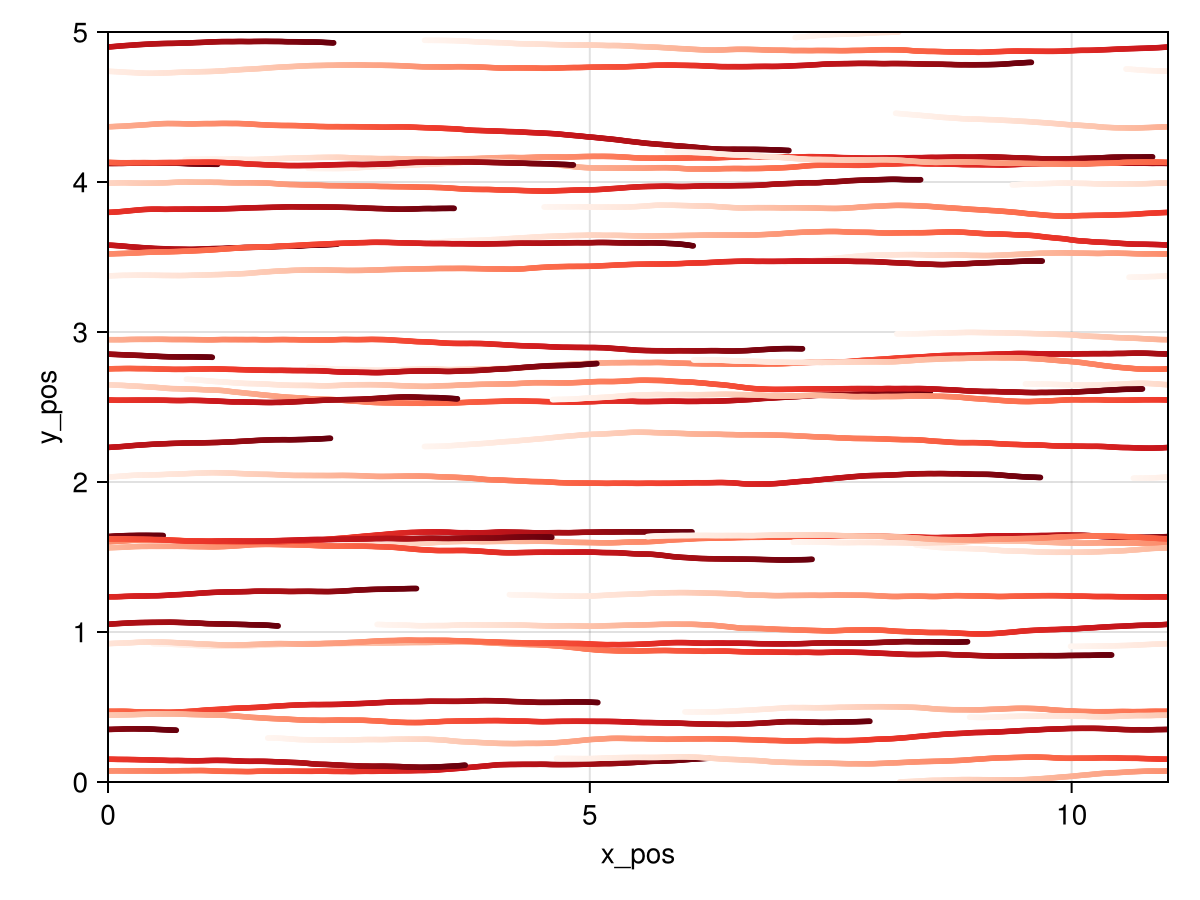
\includegraphics[width=\linewidth]{figures/st_unidflow_5000.png}
            \caption{Pedestrian trajectories for $\sigma = 0.05$}
            \label{plot:stoc_uni_traj}
        \end{subfigure}
        \caption{Unidirectional flow with stochastic effects}
        \label{plot:stoc_uni}
    \end{figure}
    With $\sigma = 0$ being the deterministic case, and $\sigma > 0$ as the non-deterministic cases. We can observe that increasing the volatility in the dynamics perturbs the velocity of the pedestrians in the unidirectional case. The effects of the randomness are as expected; the dynamics deviate more when the volatility is high.
    \pagebreak
    \item \textbf{Cross flow ($\sigma \geq 0$)}
    \begin{figure}[H]
        \centering
        \begin{subfigure}{.49\textwidth}
            \centering
            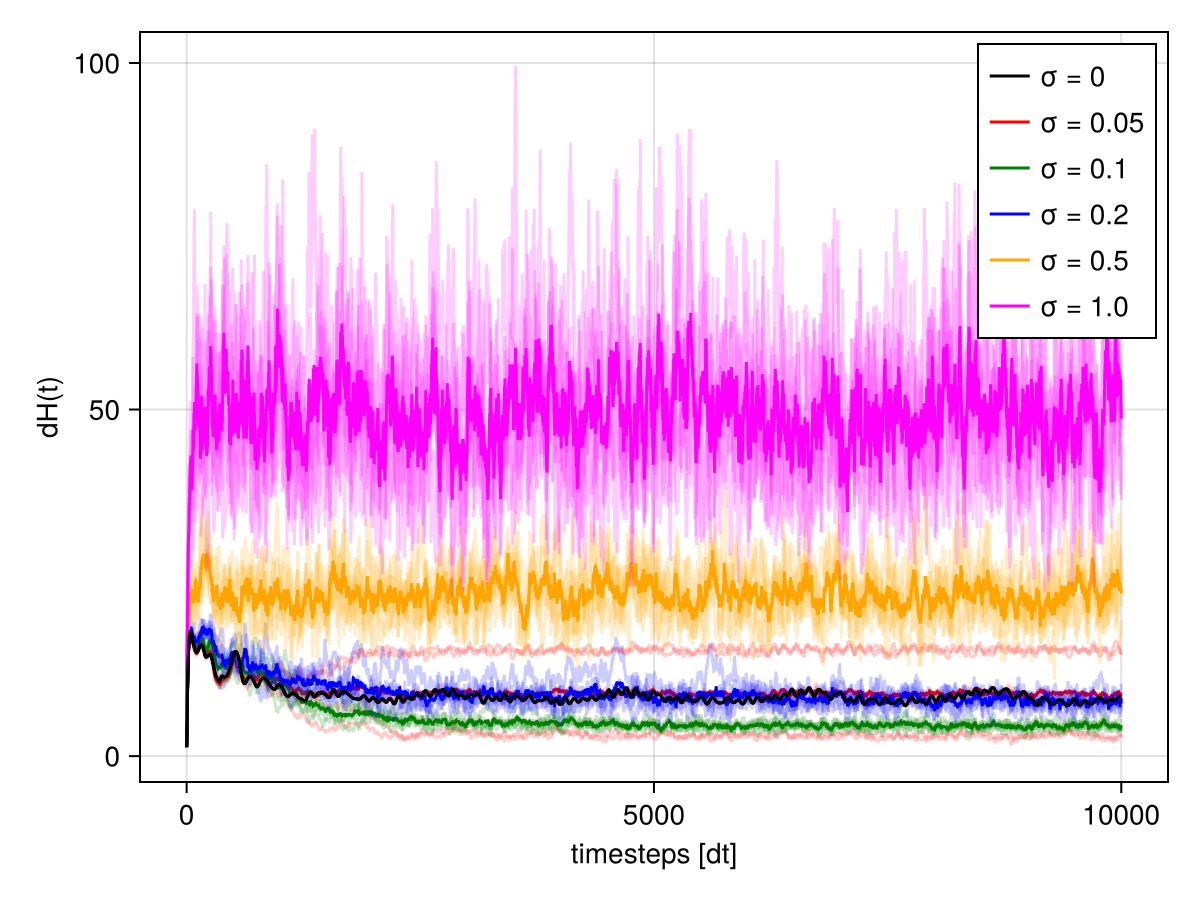
\includegraphics[width=\linewidth]{figures/dH_stochasic_cross_sigmaxy.png}
            \caption{$\frac{d}{dt}H$ over time}
            \label{plot:stoc_cross_dh}
        \end{subfigure}
        \begin{subfigure}{.49\textwidth}
            \centering
            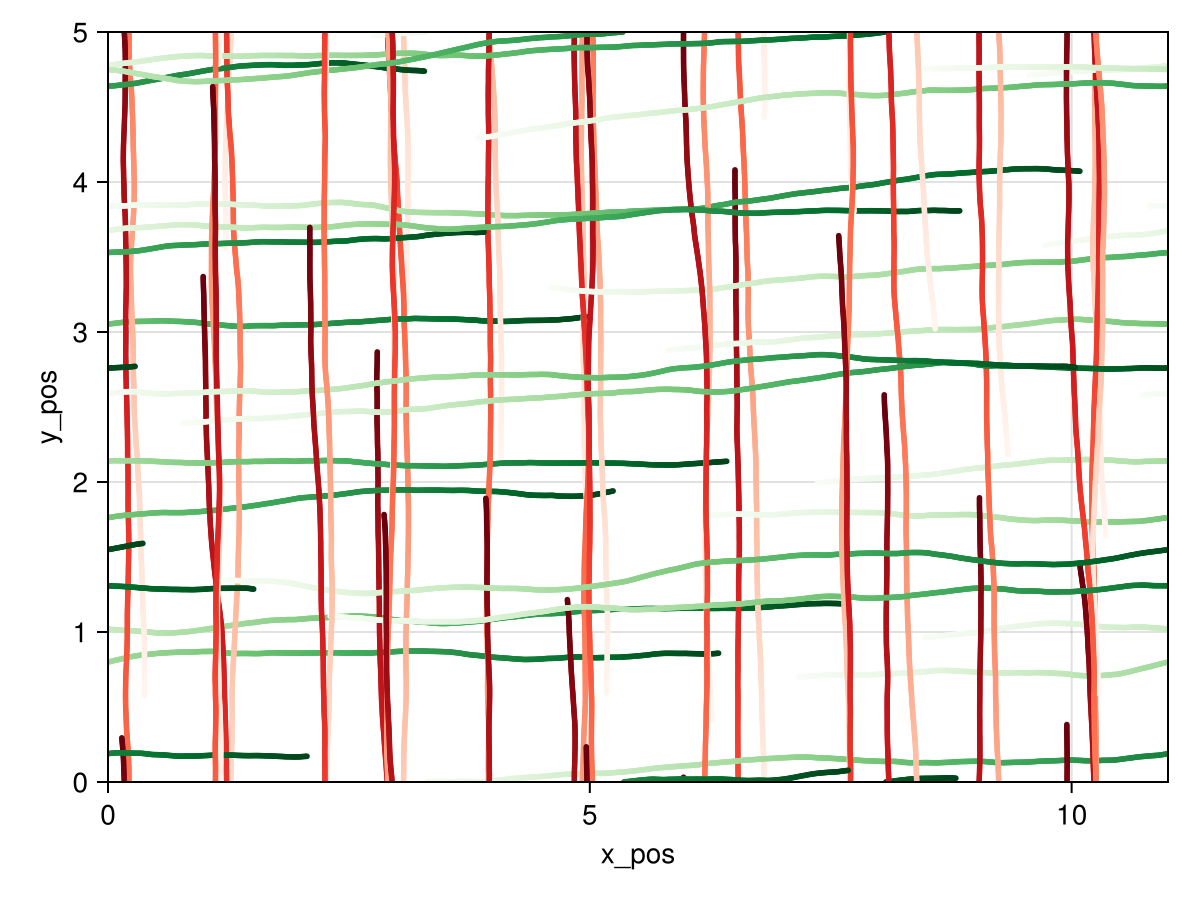
\includegraphics[width=\linewidth]{figures/s0.1_crossflow_10000.png}
            \caption{Pedestrian trajectories for $\sigma = 0.1$}
            \label{plot:stoc_cross_traj}
        \end{subfigure}
        \caption{Cross flow with stochastic effects, showing that the stripe formation improves with noise levels $\sigma \leq 0.2$}
        \label{plot:stoc_cross}
    \end{figure}
    For cross flows, the stochastic dynamics produce interesting results. For smaller values of $\sigma\geq 0$, the change of rate of the Hamiltonian is even less than the deterministic case. For such values $\sigma \leq 0.2$, as indicated in \cite{khelfa2021initiating}, the trajectories of the pedestrians also show that the stripe formation is improved with the addition of noise in contrast to its deterministic counterpart \autoref{plot:cross2}. This counterintuitive phenomenon for the stochastic cross flow is known as 'noise-induced ordering' \cite{d2021canard}. However, this stripe formation is disrupted with increase in noise, particularly for values $\sigma \geq 0.5$
    \item \textbf{Counter flow ($\sigma \geq 0$)}
    \begin{figure}[H]
        \centering
        \begin{subfigure}{.49\textwidth}
            \centering
            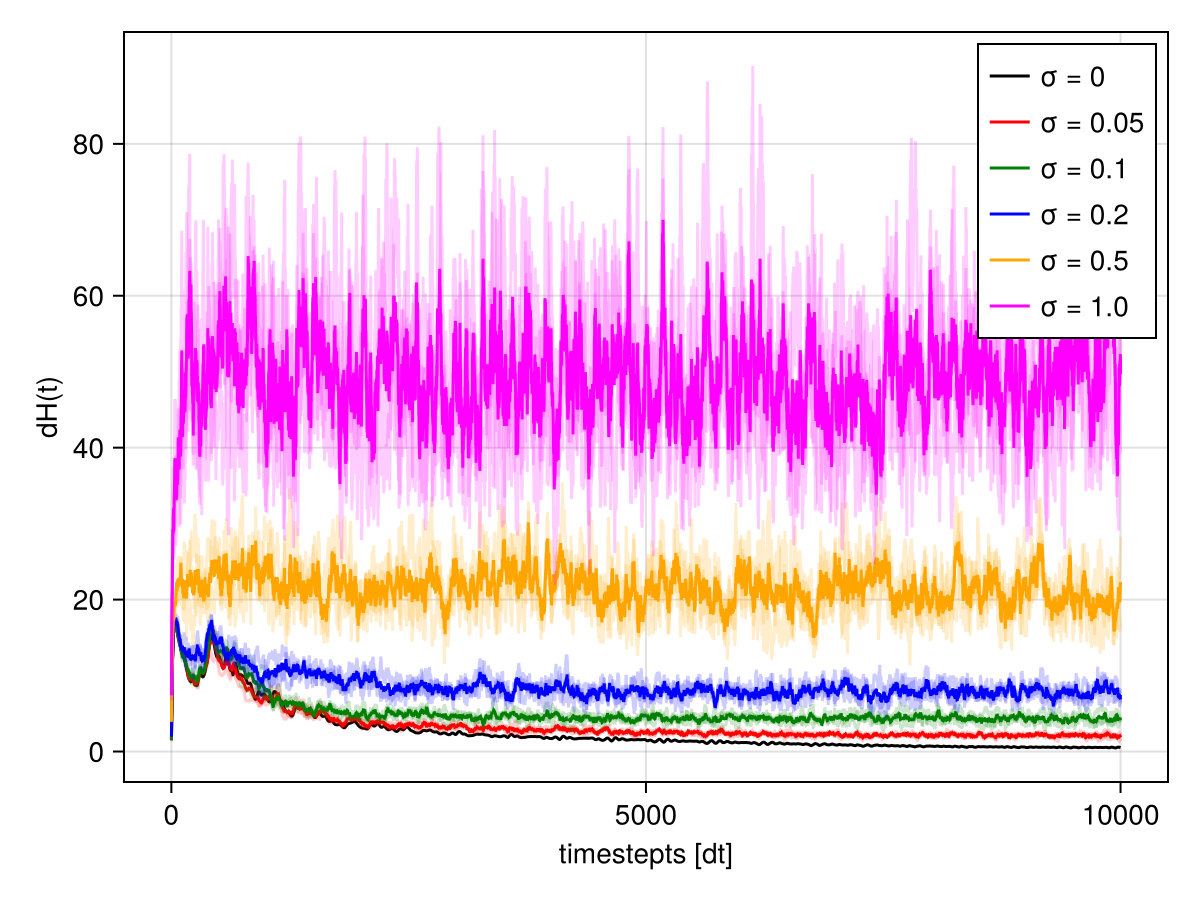
\includegraphics[width=\linewidth]{figures/dH_stochasic_counter.png}
            \caption{$\frac{d}{dt}H$ over time}
            \label{plot:stoc_counter_dh}
        \end{subfigure}
        \begin{subfigure}{.49\textwidth}
            \centering
            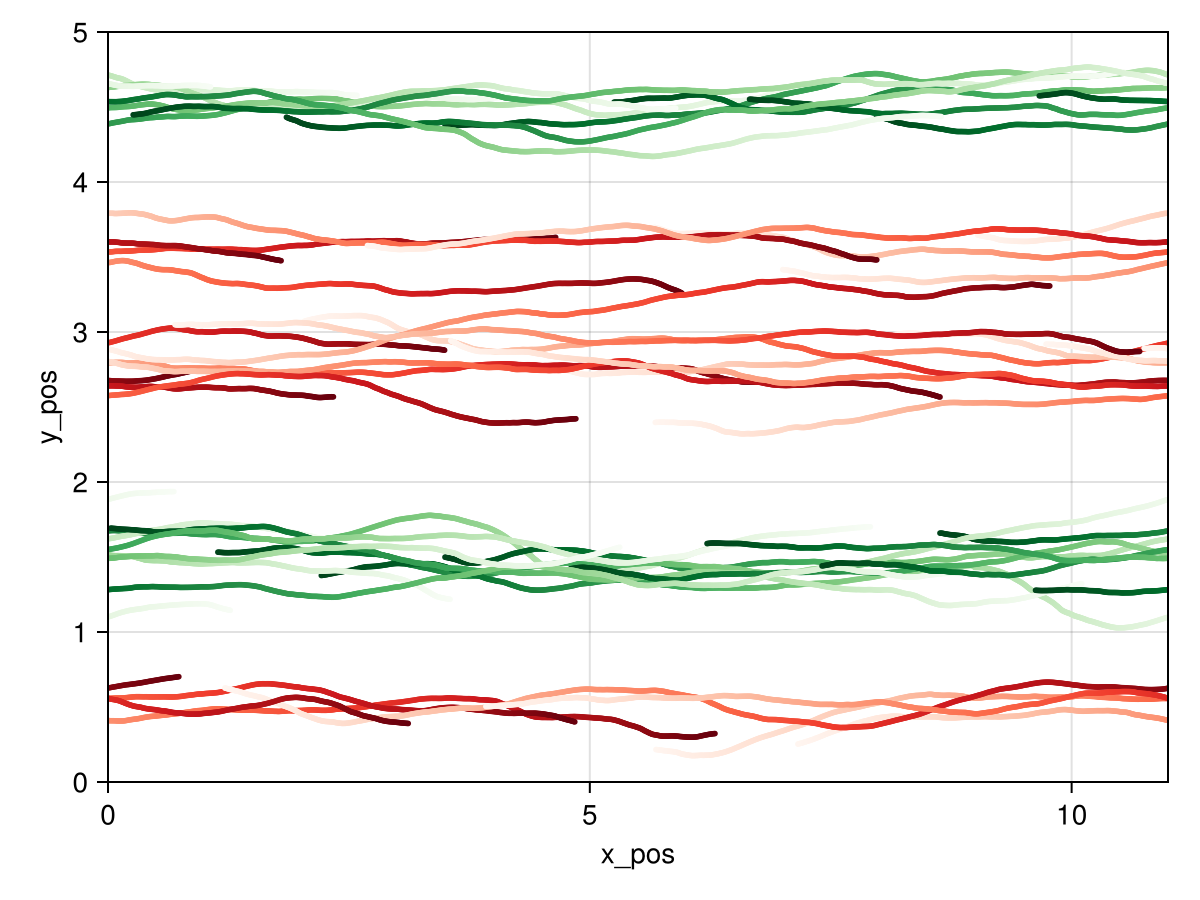
\includegraphics[width=\linewidth]{figures/s0.2_counterflow_10000.png}
            \caption{Pedestrian trajectories for $\sigma = 0.2$}
            \label{plot:stoc_counter_traj}
        \end{subfigure}
        \caption{Counter flow with stochastic effects}
        \label{plot:stoc_counter}
    \end{figure}
    In the case of the counter flow, however, we do not see an improvement in lane formation with addition of noise in the system. The lane formation is perturbed with the increase in noise and becomes indistinguishable from disordered movement when $\sigma \geq 0.5$. As the velocities of the pedestrian is decreasing here, it can be noted that this an onset of a phenomenon known as 'freezing by heating' \cite{helbing2000freezing}.
\end{itemize}

All the dynamics shown in this section, have the overall Hamiltonian greater than $H^*$, however the collective dynamics does not necessarily occur even when this condition is met in the stochastic cases, specially for the cases with high levels of noise. This could be because the rate of change of the Hamiltonian $\frac{d}{dt}H$ rapidly fluctuates, indicating erratic movement of the overall dynamics of the agents, resulting in no phase changes from disordered to ordered dynamics.


